\title{Quarks to Cosmos: Particles and Plasma in\\ 
 Cosmological Evolution}

\author{
Jeremiah Birrell\inst{1}, %\fnmsep\thanks{\email{jeremey.birrell@gmail.com}},
%Shelbi J. Foster\inst{1}, %\fnmsep\thanks{\email{shelbijfoster@arizona.edu}}, 
Christopher Grayson\inst{1}, %\fnmsep\thanks{\email{chrisgray1044@arizona.edu}},
Johann Rafelski\inst{1}%
\fnmsep\thanks{Corresponding author%\email{rafelski@gmail.com}}, 
\email{johannr@arizona.edu}}, 
%\fnmsep\thanks{\email{johannr@arizona.edu}}
\newline Andrew Steinmetz\inst{1}, %\fnmsep\thanks{\email{ajsteinmetz@arizona.edu}}
Cheng Tao Yang\inst{1}
%\fnmsep\thanks{\email{chengtaoyang@arizona.edu}}
}

\institute{Department of Physics, The University of Arizona, Tucson, AZ, 85721, USA
}

\abstract{We describe in the context of the particle physics (PP) standard model (SM) `PP-SM' the understanding of the primordial properties and composition of the Universe in the temperature range $130\GeV>T>20\keV$. The Universe evolution is described using FLRW cosmology. We present a global view on particle content across time and describe the different evolution eras using deceleration parameter $q$. In the considered temperature range the unknown cold dark matter and dark energy content of $\Lambda\mathrm{CDM}$ have a negligible influence allowing a reliable understanding of physical properties of the Universe based on PP-SM energy-momentum alone. We follow the arrow of time in the expanding and cooling Universe: After the PP-SM heavies $(t, H, W, Z)$ diminish in abundance below $T\simeq 50\GeV$, the PP-SM plasma in the Universe is governed by the strongly interacting Quark-Gluon content. Once the temperature drops below $T\simeq 150\MeV$, quarks and gluons hadronize into strongly interacting matter particles comprising a dense baryon-antibaryon content. Rapid disappearance of baryonic antimatter ensues, which adopting the present day photon-to-baryon ratio completes at $T_\mathrm{B}=38.2\MeV$. We study the ensuing disappearance of strangeness and mesons in general. We show that the different eras defined by particle populations are barely separated from each other with abundance of muons fading out just prior to $T=\mathcal{O}(2.5)\MeV$, the era of emergence of the free-streaming neutrinos. We develop methods allowing the study of the ensuing speed of the Universe expansion as a function of fundamental coupling parameters in the primordial epoch. We discuss the two relevant fundamental constants controlling the decoupling of neutrinos. We subsequently follow the early Universe as it passes through the hot dense electron-positron plasma epoch. The high density of positron antimatter disappears near $T=20.3\keV$, well after the Big Bang nucleosynthesis era: Nuclear reactions occur in the presence of a highly mobile and relatively strongly interacting electron-positron plasma phase. We apply plasma theory methods to describe the strong screening effects between heavy dust particle (nucleons). We analyze the paramagnetic characteristics of the electron-positron plasma when exposed to an external primordial magnetic field.}
\maketitle
%%%%%%%%%%%%%%%%%%%%%%%%%%%%%%%%%%%%%%%
%\setcounter{\thesubsection}{1}
%\stepcounter{\thesubsection}
\newpage
%\setcounter{secnumdepth}{3}
%\setcounter{tocdepth}{2}
\setcounter{tocdepth}{3}
\tableofcontents
%%%%%%%%%%%%%%%%%%%%%%%%%%%%%%%%%%%%%%%

%%%%%%%%%%%%%%%%%%%%%%%%%%%%%%%%%%%%%%% 
\section{Introduction}
%%%%%%%%%%%%%%%%%%%%%%%%%%%%%
\subsection{Theoretical models of the primordial Universe}\label{ssec:UniLab}
\paragraph{Connecting prior works:}
In this report we explore the connection between particle, nuclear, and plasma physics and the evolution of the Universe in the domain described by laws of physics we learned about in laboratory experiments.

The question we address is how a very hot soup of elementary matter evolves and connects to the normal matter in the era of the Big-Bang nucleosynthesis. We present here the theoretical insights gained over the past dozen years in an effort to create a backdrop of knowledge allowing to seek any remnant observables accessible today.

We expand considerably both in scope and content our recent review~\cite{Rafelski:2023emw}. However, this report is not a traditional review: We collect here in heavily edited and re-sequenced manner selected material from the contents of four Ph.D. Thesis completed at the Department of Physics, The University of Arizona by:
\begin{enumerate}
\item Jeremiah Birrell~\cite{Birrell:2014ona},
\item Christopher M. Grayson~\cite{Grayson:2024okq},
\item Andrew J. Steinmetz~\cite{Steinmetz:2023ucp}, and
\item Cheng Tao Yang~\cite{Yang:2024ret}.
\end{enumerate}
Due to graduation time constraints some of this presented material is only found in follow-up publications, see the list below. The context of strong interactions and quark-gluon plasma hadronization in the Universe was studied before:
\begin{enumerate}
\item[5.] Essential for the presentation material from the prior research work  which describes our understanding about: i) deconfined state of hot quarks and gluons, the quark gluon plasma (QGP); and ii) hot hadronic phase of matter, as applicable to the context of the early Universe~\cite{Rafelski:2015cxa,Rafelski:2016hnq,Letessier:2002ony}.
\end{enumerate}
%%%%%%%%%%%%%%%%%%%%%%%%%%%%%%%%%%%%%%%%%%
As noted we rely in this report also on our  research papers and reports including:
\begin{enumerate}
\item {\small ``Self-consistent Strong Screening Applied to Thermonuclear Reactions''}~\cite{Grayson:2024uwg} (preprint 2024) We explore the strong screening effects in BBN epoch due to dynamic and nonlinear polarization of the matter-antimatter (electron-positron) ambient medium.
%
 \item ''A Short Survey of Matter-Antimatter Evolution in the Primordial 
Universe'' by~\cite{Rafelski:2023emw} (2023) is a prequel to this review  focused on the role of positron-antimatter in the early universe. 
%
\item ''Matter-antimatter origin of cosmic magnetism'' 
by~\cite{Steinmetz:2023nsc} (2023) proposes a model of para-magnetization driven by the large 
matter-antimatter (electron-positron) content of the early universe allowing for the first time in this context for spin magnetism.
%
\item ''Electron-positron plasma in BBN: Damped-dynamic screening'' by~\cite{Grayson:2023flr} (2023) employs the linear response theory to describe the inter-nuclear potential screened by in electron-positron pair plasma in the BBN epoch. This work includes the computation of the chemical potential and plasma damping rate required in semi-analytical study of the relativistic Boltzmann equation in the context of the linear response theory.  
%
\item ``Dynamic magnetic response of the quark-gluon plasma to electromagnetic fields''~\cite{Grayson:2022asf} (2022) The linear response theory is applied to quark-gluon plasma environment in presence of strong magnetic fields.
%
\item ''Cosmological Strangeness Abundance'' by~\cite{Yang:2021bko} (2021) presents our complete  study of the strange particle composition in the expanding primordial  Universe includijng determination of various  freeze-out temperatures.
%
\item ``Current-conserving Relativistic Linear Response for Collisional Plasmas''~\cite{Formanek:2021blc} (2021) develops relativistic linear response plasma theory implementing conservation laws, obtaining general solutions and laying foundation for applications to primordial Universe plasma conditions.
%
\item ''The Muon Abundance in the Primordial Universe'' by~\cite{Rafelski:2021aey} (2021) is a conference proceedings paper dedicated to exploration of  muon abundance and its persistence temperature in the primordial Universe. 
%
\item ''Reactions Governing Strangeness Abundance in Primordial Universe''~\cite{Rafelski:2020ajx}  (2020) is a conference proceeding paper whichlays ground work for the study of strangeness reactions in the primordial Universe. 
%
\item''Possibility of bottom-catalyzed matter genesis near to primordial QGP hadronization''~\cite{Yang:2020nne} (preprint 2020) has been our fist study of the bottom flavor abundance and show the  nonequilibrium behavior near to QGP hadronization. 
%
\item ''Lepton Number and Expansion of the Universe''~\cite{Yang:2018oqg} (preprint 2018) proposes a model of large lepton asymmetry and explore how this large cosmological lepton yield
relates to the effective number of (Dirac) neutrinos.
%
\item''Temperature Dependence of the Neutron Lifespan''~\cite{Yang:2018qrr} (preprint 2018) is a study of neutron lifespan in plasma with Fermi-blocking from electron and neutrino. 
%
\item ''Strong fields and neutral particle magnetic moment dynamics''~\cite{Formanek:2017mbv} (2017) was an overview of our early research group's efforts in studying neutral particle dynamics in electromagnetic fields. It includes a neutrino section. 
%
\item ``The hot Hagedorn Universe''~\cite{Rafelski:2016cho} (2016) is a short conference report recounting the impact of Hagedorn work on phase transformation at Hagedorn temperature in primordial Universe, updating these results to modern context.
%
\item "Relic Neutrino Freeze-out: Dependence on Natural Constants"~\cite{Birrell:2014uka} (2014) is a study of neutrino freeze-out temperature as a function of standard model parameter and its application on the effective number of (Dirac) neutrinos. This reference provides all   neutrino-matter weak interaction matrix elements required for the Boltzmann code. 
%
\item ``Quark–gluon Plasma as the Possible Source of Cosmological Dark Radiation''~\cite{Birrell:2014cja} (2014) explores the role of dark radiation created at time of QGP hadronization in accelerating Universe today.
%
\item ``Boltzmann Equation Solver Adapted to Emergent Chemical Non-equilibrium''~\cite{Birrell:2014gea} (2014) addresses the transport theory tools we developed to charcterize the slow in time freeze-out of neutrinos in primordial Universe.
%
\item ``Proposal for Resonant Detection of Relic Massive Neutrinos''~\cite{Birrell:2014qna} (2014) characterizes the primordial neutrino flux spectrum today and explores experimental approaches for experimental observations.
%
\item ``Traveling Through the Universe: Back in Time to the Quark-Gluon Plasma Era''~\cite{Rafelski:2013yka} (2013) presents a conference report on the connection between quark-gluon plasma and neutrino freeze-out epochs.
%
\item ``Connecting QGP-Heavy Ion Physics to the Early Universe''~\cite{Rafelski:2013qeu} (2013) Explores in a conference setting the properties of the primordial Universe at QGP hadronization and connects to the ongoing experimental heavy ion effort to study the hadronization process.
%
\item ''Fugacity and Reheating of Primordial Neutrinos'' by~\cite{Birrell:2013gpa} (2013) is as study of neutrino fugacity as a funciton of neutrino kinetic freeze-out temperature. This short work includes neutrino interaction matrix  elements and is helping the evaluation of  neutrino relaxation time. 
%
\item ''Relic Neutrinos: Physically Consistent Treatment of Effective Number of Neutrinos and Neutrino Mass''~\cite{Birrell:2012gg}  (2012) is a model independent study of the neutrino momentum distribution at freeze-out, treating the freeze-out temperature as a free parameter.
%
\item ``From Quark-Gluon Universe to Neutrino Decoupling: $200 < T < 2$\,MeV''~\cite{Fromerth:2012fe} (2012) Conference report presenting a first review connecting  the Quark-Hadron phase transformation and neutrino decoupling as a function of current era cosmologicall properties.
%
\item ``Unstable Hadrons in Hot Hadron Gas in Laboratory and in the Early Universe''~\cite{Kuznetsova:2010pi} (2010) Shows that some unstable hadrons may persist in evolution of the Universe as the detailled balance condition is never broken due to strong coupling to the photon background.
%
\item ``Hadronization of the Quark Universe''~\cite{Fromerth:2002wb} (preprint 2002) First detailled study of chemical potentials and conditions of hadronization of QGP in primordial Universe.
%
%\item ``Hadrons and Quark–Gluon Plasma''~\cite{Letessier:2002ony} (2002) Introductory chapters in this textbook connect the field of relativistic heavy ions to the properties of primordial Universe. 
\end{enumerate}

It is our hope that this collection of material allows the reader to obtain a smooth connection in the entire spplicable temperature domain $130\,\mathrm{GeV}>T>20\,\mathrm{keV}$.

\paragraph{Dominance of visible matter in primordial Universe:}
In this report, we aim to connect various eras of cosmological evolution which can be addressed with some confidence in view of the already known particle and nuclear properties as measured experimentally. By analyzing the early Universe as a function of time we are exploring the role of particle physics standard model (PP-SM) in the Universe evolution. We snapshot in this report specific epochs in primordial Universe, or/and on specific physical conditions such as primordial magnetic fields.

In the cosmic epoch considered here with temperature above $kT=20$\,keV the present day dominant dark matter and dark energy played a negligible role in the cosmos. The changing composition of the Universe is illustrated in \rf{fig:energy_frac}. To create the figure we integrate the Universe backwards in time, the assumed composition of the Universe in current era is: $69\%$ dark energy, $26\%$ dark matter, $5\%$ baryons,  photons and neutrinos make less than one percent in current era; we further assumed one  massless neutrino and two with $m_\nu=0.1$\,eV, other neutrino mass values are possible, constraints remain weak.

%%%%%%%%%%%%%%%%%%%%%%%%%%%%%%%%%%%%
\begin{sidewaysfigure}
\vspace*{0.62\textwidth}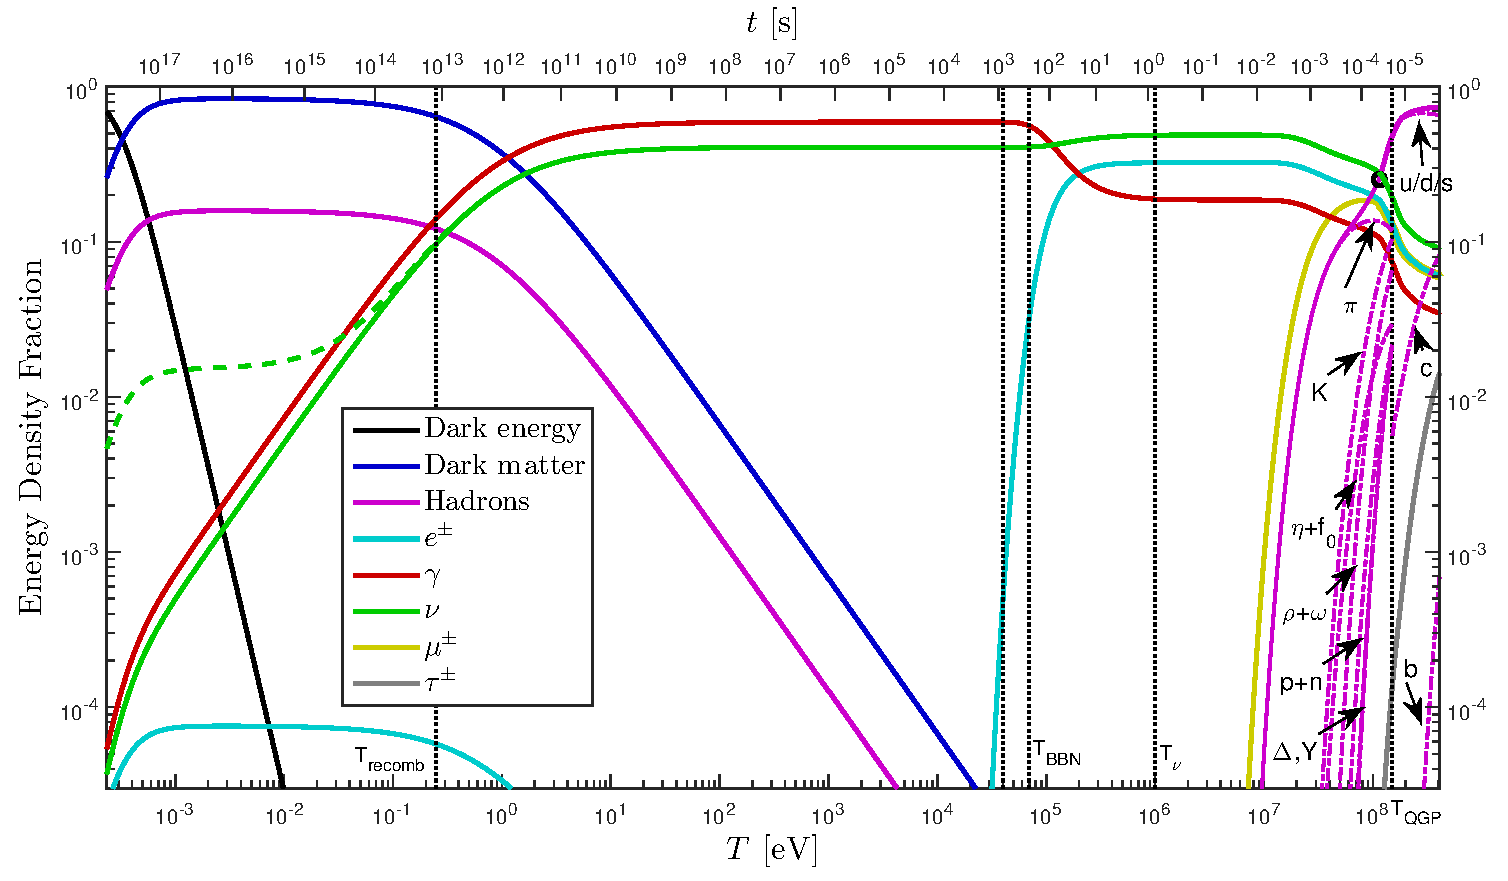
\includegraphics[width=\textwidth]{01-introduction/Figures/energyFractions.pdf}\label{fig:energy_frac}
\caption{Evolving in time  fractional  energy composition of the Universe. Expanded from the thesis of J.\,Birrell~\cite{Birrell:2014ona} and adopted from~\cite{Rafelski:2023emw}}
 \end{sidewaysfigure}
%%%%%%%%%%%%%%%%%%%%%%%%%%%%%%%%%%

As described there are two unknown dark components as one is able to disentangle their behavior given two inputs in the energy-momentum tensor, pressure and energy density, which are related by equations of state. The current epoch comic accelerated expansion (Nobel price 2011 to Saul Perlmutter, Adam Riess, and Brian P. Schmidt) creates the need for two component ``darkness''.

Dark energy in conventional definition is akin to $\Lambda$=Einstein's cosmological term. $\Lambda$ is a fixed property of the Universe and does not scale with temperature. In comparison radiation energy content scales with $T^4$ and is vastly dominant in the temperature range we explore. Cold {\it i.e.\/} dark matter (CDM) content scales with $T^{3/2}$ for $m/T\gg 1$. In the temperature regime of interest to us CDM complements the invisible normal baryonic matter. The further back we look at the hot Universe, the more irrelevant become all form of matter including ``dark'' matter component. 

There is considerable tension between studies determining the present day speed of cosmic expansion (Hubble parameter)~\cite{DiValentino:2024spr,DiValentino:2021izs}: Extrapolation from the distant past, {\it i.e.\/} recombination epoch near red shift $z=1000$, are smaller than the Universe properties observed and studied in the current epoch a result stated often asking the question "67 or 75?". This unresolved issue arises from the epochs when the Universe was in its atomic, molecular, stellar forms which is in principle irrelevant to our particle and plasma study of the Universe. However, this separation of scales maybe not complete as we will argue. Depending on details of PP-SM in the neutrino sector, free streaming neutrinos contribute to darkness and may impact on what exactly is the result of extrapolation ("67 or 75?") of Hubble expansion from recombination epoch to the current epoch. One could argue that the effort to study the "Unknown" darkness in cosmology suffers from the lack of full understanding of the "Known" in the primordial cosmos which mascarades as darkness today. This is one of many motivations for the research effort we pursue. 

 
%%%%%%%%%%%%%%%%%%%%%%%%%%%%%%%%%%%%%%%%%%
\paragraph{Cosmic plasma in the early Universe:}
%\label{ssec:plasmas}
%In this section we will focus on the following:
%\begin{itemize}
% \item Five different plasma epoch from $0.3\mathrm{GeV}>T>20$keV
%\end{itemize}

%We present an overview of the Universe evolution as a function of temperature from $300\,\mathrm{MeV}>T>0.02\,\mathrm{MeV}$ and main events constituting the history of the early Universe as seen 


The primordial hot Universe fireball underwent several nearly adiabatic phase changes that dramatically evolved its bulk plasma properties as it expanded and cooled in the temperature range $300\,\mathrm{MeV}>T>0.02\,\mathrm{MeV}$ ~\cite{Rafelski:2023emw}. We will address in this work four well separated domains of particle plasma and two topical plasma challenges. After the electroweak symmetry breaking sets in,  the comic plasma in the early Universe evolves in the first hour down to temperature of about $T\simeq 10\keV$. Notable plasma conditions include:
\begin{enumerate}
\item \textbf{Primordial quark-gluon plasma epoch:}  
At early times when the temperature was between $130\,\mathrm{GeV}>T>0.15\,\mathrm{GeV}$ we have in the primordial plasma in their thermal abundance all PP-SM  building blocks of the Universe as we know them today, including the Higgs particle, the vector gauge electroweak and strong interaction bosons, all three families of leptons and free deconfined quarks. Clearly as temperature decreases below heavy particle mass the thermal abundance is much reduced. In fact near to the QGP phase transition $300\, \mathrm{MeV}>T>150$ MeV, the bottom quark breaks the detail balance and disappearance from particle inventory provides the arrow in time, see \rsec{Bottom} for further discussion. 
%As all hadrons are dissolved into their constituents during this time, strongly interacting particles $u,d,s,t,b,c,g$ controlled the fate of the Universe.
%
\item \textbf{Hadronic epoch:}  Around the hadronization temperature $T_H\approx150\,\mathrm{MeV}$, a phase transformation occurred, forcing the free quarks and gluons to become confined within baryon and mesons; experimental results confirming the universal nature of the hadronization process were described in Ref.\,\cite{Letessier:2005qe}. In the temperature range $ 150\,\mathrm{MeV}>T>20\,\mathrm{MeV}$, the Universe is rich in physics phenomena involving strange mesons and (anti)baryons including (anti)hyperon abundances~\cite{Fromerth:2012fe,Yang:2021bko}. The antibaryons disappear from the Universe at temperature $T=38.2$ MeV, and strangeness can be produced by the inverse decay reactions that are in equilibrium via weak, electromagnetic, and strong interactions in the early Universe until $T\approx13$ MeV , see \rsec{Strangeness} for detailed discussion.
%
\item \textbf{Lepton-photon epoch:}  For temperature $10\,\mathrm{MeV}>T>2\,\mathrm{MeV}$ massless leptons and photons controlled the fate of the Universe: The Universe contained relativistic electrons, positrons, photons, and three species of (anti)neutrinos. During this epoch Massive $\tau^\pm$ disappear from the plasma at high temperature via decay processes. However, $\mu^\pm$ leptons can persist in the early Universe until temperature $T=4.2$ MeV, and positron $e^+$ can persist until the temperature $T=0.02$ MeV, see \rsec{Electron} for detailed discussion.

In this temperature epoch neutrinos were still coupled to the charged leptons via the weak interaction~\cite{Birrell:2012gg,Birrell:2014ona}, they freeze-out in the temperature range $3\,\mathrm{MeV}>T>2\,\mathrm{MeV}$, exact value depends on the neutrino's flavors and the magnitude of the PP-SM parameters, see \rsec{Neutrino} for detailed discussion. After neutrino freeze-out, they still play a important role in the Universe expansion via the effective number of neutrinos $N_{\nu}^{\mathrm{eff}}$, which relates to  the Hubble parameter value in current epoch.
%
\item \textbf{Electron-positron epoch:}  After neutrinos freeze-out at $T=3\sim2\,\mathrm{MeV}$ and become free-streaming in the early Universe, the cosmic plasma was dominated by electrons, positrons, and photons. The $e^\pm$ plasma existed until $T\approx 0.02\,\mathrm{MeV}$. Properties of this plasma need to be studied in order to understand the behavior of the nucleon dust also present.
%
\item \textbf{BBN occurs in the midst of ${\mathbf e^+e^-}$ plasma:} Contrary to what was the prevailing context only a few years ago, it is today understood that BBN occurred within a rich electron-positron plasma environment. There are 1000's of ${ e^+e^-}$-pairs for each nucleon undergoing nuclear BBN fusion reaction. 
%
\item \textbf{Primordial magnetism:}\index{magnetism!primordial} The $e^{+}e^{-}$-plasma (electron-positrons pairs) at temperatures reaching well below BBN epoch in the primordial universe could be a source of the present day intergalactic magnetic fields. See \rsec{Electron} for detailed discussion. We explore Landau diamagnetic and magnetic dipole moment paramagnetic properties. A relatively small magnitude of the $e^{+}e^{-}$ magnetic moment polarization asymmetry suffices to produce a self-magnetization in the universe consistent with present day observations.
\end{enumerate}

After $e^\pm$ annihilation finishes at a temperature near 20keV, the Universe was still opaque to photons due to large photon-electron scattering Thompson cross section. Observational cosmology study of the Cosmic Microwave Background (CMB)~\cite{Planck:2018vyg} addresses the epoch of free electron binding into atoms -- a process referred to as recombination. This is complete at $T_\mathrm{recomb}\approx 0.25\,\mathrm{eV}$. 

%%%%%%%%%%%%%%%%%%%%%%%%%%%%%%%%%
\paragraph{Towards experimental study of primordial particle Universe:} Just before quarks and gluons were adopted widely as elementary degrees of freedom in PP-SM, the so-called `Lee-Wick' model of dense primordial matter prompted a high level meeting: The Bear Mountain November 29-December 1, 1974 meeting had decisive impact on the development of the research program leading to the understanding of primordial particles in the Universe. This meeting was not open to all interested researchers: Only a few dozen were invited to join the participant club, see last page of the meeting report: \url{https://www.osti.gov/servlets/purl/4061527}. This is an unusual historical fact witnessed by one of us (JR), for further discussion see Ref.\,\cite{Rafelski:2019twp}. 

It is noteworthy that our report appears in essence on the 50th year anniversary of this 1974 meeting. Within just half a century the newly developed PP-SM knowlege has rendered all but one insight of the 1974 meeting obsolete: The participating representatives of particle and nuclear physics elite of the epoch recognized the novel opportunity to experimentally explore hot and dense hadron (strongly interacting) matter by colliding high energy nuclei (heavy ions). One of the participants, Alfred Goldhaber, planted in the Nature magazine~\cite{Goldhaber:1978qp} the seed which grew into the RHIC collider at BNL-New York. 

%%%%%%%%%%%%%%%%%%%%%%%%%%%%%%%%%
\paragraph{Phase transformation in the primordial Universe:} Thanks to tireless effort of Rolf Hagedorn~\cite{Rafelski:2016hnq} the European laboratory CERN was intellectually well positioned for the rapid development of related physics ideas and the required experimental program. A major physics motivation that soon emerged was the understanding of the primordial composition of the hot Universe. The pre-1970 idea advanced by Hagedorn, by Huang and Weinberg~\cite{Huang:1970iq} and in the following by many others was that the Universe was bound to a maximum Hagedorn temperature of $kT\le kT_H=150-180$\,MeV at which the energy content diverged. In the following years and indeed by the time of the Bear Mountain meeting the idea that a symmetry restoring change in phase structure would develop at finite temperature was already taking hold~\cite{Weinberg:1974hy,Harrington:1974fc}.

Today we understand Hagedorn temperature $T_H$ to be the phase transformation to the deconfined phase of matter where quarks and gluons can exist. The first clear statement about the existence of a phase boundary connecting Hagedorn hadron gas with constituent quarks invoking deconfinement at high temperature was the 1975 work of Cabibbo and Parisi~\cite{Cabibbo:1975ig}, which was followed by a more quantitative characterization within the realm of the MIT bag model of hadrons by~\cite{Chin:1978gj} and soon after by Rafelski and Hagedorn incorporating Hagedorn bootstrap model of hadronic matter, see Ref.\,\cite{Rafelski:2015cxa} and appendices A and B therein. This work implemented as well as was at that time possible using a model the Cabibbo-Parisi proposal in all detail.

Could deconfined state of a hot phase of quarks and gluons we call QGP really exist beyond Hagedorn temperature? A broad acceptance of this new insight took decades to take hold. Many works in 1970's epoch missed the need to smoothly connect quarks to hadrons incorporating gluons. Neglecting, or omitting the gluonic degrees of freedom pushed the transformation temperature towards $T=400$\,MeV, creating glaring conflict with well established Hagedorn hadronic phase temperature limit $T_H\simeq 160\pm 10$\,MeV. Yet other large body of work in this epoch addressed at zero temperature the dissolution of hadrons at ultra high density into quark constituents of astrophysical interest, without relevance to the understanding of both the early Universe and the relativistic heavy ion collisions.

These two fields, primordial Universe and ultra relativistic heavy ion collisions relate to each other very closely. There is little if any relation to dense neutron matter found in compact stars. Super-novae explosions crate at much lower matter density temperatures reaching above 50\,MeV. The ongoing laboratory work at CERN-LHC and BNL-RHIC exploring the physics of QGP in the high temperature and high particle density regime allows study of elementary strongly interacting matter  connecting quarks to cosmos.
 
Can we really tell apart in these ultra relativistic heavy ion experiments the  two different phases of matter? In the end the outcome seems to be the same, conversion of colliding nuclei energy into many material particles. This question haunted this field of research for decades~\cite{Rafelski:2015cxa,Harris:2024aov}, a topic which is not addressed in this work beyond the following few words: 

The collision micro-bang involves time scales which are about 16 orders of magnitude shorter compared to the characteristic scale governing the Universe Big-Bang. When one of us (JR) first arrived at CERN in 1977, he found himself immersed into ardent discussions about both what the structure of the hot primordial Universe could be and if indeed we could figure out the answer in an experiment: Was the Universe  perhaps a dense baryon-antibaryon universe? Or was indeed the confinement condition not really retained at high temperature~\cite{Weinberg:1974hy,Harrington:1974fc,Cabibbo:1975ig}? And above all, how can we tell doing laboratory experiments? By 1979 it became clear that new ideas about experimental observables were needed based on specific properties of the dense hot matter if formed in experiments. Strange antibaryon enhancement was one of the proposed novel approaches and in the opinion of one of us (JR), this was to be later the decisive QGP discovery evidence.

%%%%%%%%%%%%%%%%%%%%%%%%%%%%%%%%%%%%%%%%%%%%%%
\subsection{Concepts in statistical physics} \label{sec:statphys}
We now introduce the fundamental statistical physics concepts necessary to explore the properties of the Universe during its 'first hour'. In the case of local thermal equilibrium, the laws of thermodynamics can provide a framework for understanding the behavior of particle's energy density, pressure, number density and entropy in the early Universe.

We will address the general Fermi and Bose distributions and its application in the early Universe, as well as the thermodynamics of the early Universe. As before we use natural units $c=\hbar=k_{B}=1$. We also explore case of free streaming particles and possibility of freeze-out conditions {\it i.e.\/} rise of non-equilibrium abundance.

%%%%%%%%%%%%%%%%%%%%%%%%%%%%%
\paragraph{Quantum statistical distributions}
\index{Statistical distribution}
In the early Universe, the reaction rates of particles in the cosmic plasma were much greater than the Universe expansion rate $H$. Therefore, the local thermal equilibrium has been maintained. Assuming the particles are in thermal equilibrium, the dynamical information can be obtained from the single-particle distribution function. The general relativistic covariant Fermi/Bose momentum distribution can be written as
\begin{align}
f_{F/B}(\Upsilon_i,p_i)=\frac{1}{\Upsilon^{-1}_i\exp{\left[(u\cdot p_i-\mu_i)/T\right]}\pm1}
\end{align}
where the plus sign applies for fermions, and the minus sign for bosons. The Lorentz scalar $(u_i\cdot p_i)$ is a scalar product of the particle four momentum $p^\mu_i$ with the local four vector of velocity $u^\mu$. In the absence of local matter flow, the local rest frame is the laboratory frame 
\begin{align}
u^\mu=\left(1,\vec{0}\right),\,\,\,\,\,\,\,\,\, p^\mu_i=\left(E_i,\vec{p}_i\right).
\end{align}  
The parameter $\Upsilon_i$ is the fugacity of a given particle which describes the pair density and it is the same for both particles and antiparticles. For $\Upsilon_i=1$ the distribution maximizes the entropy content at a fixed particle energy. The parameter $\mu_i$ is the chemical potential for a given particle which is associated to the density difference between particles and antiparticles. 

%%%%%%%%%%%%%%%%%%%%%%%%%%
\paragraph{Chemical equilibrium:}
In general there are two types of chemical equilibriums associated with the chemical parameters $\Upsilon$ and $\mu$. We have:
\begin{itemize}
\item Absolute chemical equilibrium:\\
The absolute chemical equilibrium is the level to which energy is shared into accessible degrees of freedom, e.g. the particles can be made as energy is converted into matter.
The absolute equilibrium is reached when the phase space occupancy approaches unity $\Upsilon\to1$. 
 \item Relative chemical equilibrium:\\
 The relative chemical equilibrium is associated with the chemical potential $\mu$ which involves reactions that distribute a certain already existent element/property among different accessible compounds. 
 \end{itemize}
The dynamics of absolute chemical equilibrium, in which energy can be converted to and from particles and antiparticles, is especially important. The consequences for the energy conversion to from particles/antiparticle can be seen in the first law of thermodynamics by introducing the general chemical potential $\mu_N$ for particle and $\mu_{\bar{N}}$ for antiparticle as follows:
\begin{align}
\mu_N\equiv\mu+T\ln\Upsilon,\qquad{\mu_{\bar{N}}}\equiv{-\mu}+T\ln\Upsilon.
\end{align}
Then the first law of thermodynamics can be written as
\begin{align}
dE&=-PdV+TdS+{\mu_N}dN+{\mu_{\bar{N}}}d{\bar{N}}
\\&=-PdV+TdS+{\mu}(dN-d{\bar{N}})+T\ln{\Upsilon}(dN+d{\bar{N}}).
\end{align}
It shows that the chemical potential $\mu$ is the energy required to change the difference between particles and antiparticles, and the $T\ln\Upsilon$ is the energy required to change the total number of particle and antiparticle, and the fugacity $\Upsilon$ is the parameter to adjust the energy.

%%%%%%%%%%%%%%%%%%%%%%%%%%%%%%%%%
\paragraph{Boltzmann equation and particle freeze-out}
The Boltzmann equation describes the evolution of distribution function f in phase space. The Boltzmann equation in the FLRW universe can be written as
\begin{align}
\frac{\partial f}{\partial t}-\frac{\left(E^2-m^2\right)}{E}H\frac{\partial f}{\partial E}=\frac{1}{E}\sum_{q}\mathcal{C}_q[f],
\end{align}
where $H=\dot{a}/a$ is the Hubble parameter. Due to homogeneity and isotropy of the Universe, the distribution function depends on time $t$ and energy $E=\sqrt{p^2+m^2}$ only. The collision term $\sum_qC_q$ represents all elastic and inelastic interactions and $q$ labels the corresponding physical process. In general, the collision term is proportional to the relaxation time for given collision as follows \cite{Anderson:1974nyl}
\begin{align}
\frac{1}{E}\mathcal{C}_q[f]\propto\frac{1}{\tau_{rel}}
\end{align}
where $\tau_{rel}$ is the relaxation time for the reaction, which is on the order of magnitude of time for the reaction to reach chemical equilibrium. 


As the Universe expands, the collision term in the Boltzmann equation competes with the Hubble term. In general, a given particle freeze-out from the cosmic plasma when its interaction rate $\tau_{rel}^{-1}$ becomes smaller than the Hubble expansion rate
\begin{align}
H\geqslant\tau_{rel}^{-1}.
\end{align}
When this happens, the particle's interactions are not rapid enough to maintain thermal distribution, either because the density of particles becomes so low that the chances of any two particles meeting each other becomes negligible, or because the particle energy becomes too low to interact. The freeze-out process can be categorized into three distinct stages based on the type of freeze-out interactions, we have~\cite{Birrell:2012gg,Rafelski:2023emw}:

\begin{itemize}
\item Chemical freeze-out :\\
As the Universe expands and the temperature drops, the rate of the inelastic scattering (e.g. production and annihilation reaction) that maintain the equilibrium density becomes smaller than the expansion rate. At this point, the inelastic scattering ceases, and a relic population of particles remain. Prior to the chemical freeze-out temperature, number changing processes are significant and keep the particle in thermal equilibrium, implying that the distribution function has the usual Fermi-Dirac form 
\begin{equation}\label{equilibrium}
f_{th}(t,E)=\frac{1}{\exp[(E-\mu)/T]+1},\qquad \text{ for } T(t)> T_{ch}.
\end{equation}
where $T_{ch}$ represents the chemical freeze-out temperature.\index{chemical freeze-out}


\item Kinetic freeze-out:\\
After chemical freeze-out, particles  still scatter elastically from other particles and keep thermal equilibrium in the primordial plasma. As the temperature drops, the rate of elastic scattering reaction that maintain the thermal equilibrium become smaller than the expansion rate. At that time, elastic scattering processes cease, and the relic particles do not interact with other particles in the primordial plasma anymore. Before the kinetic freeze-out, the distribution function has the form
\begin{equation}\label{kinetic_equilib}
f_k(t,E)=\frac{1}{\Upsilon^{-1}\exp[(E-\mu)/T]+1},\qquad \text{ for }T_f< T(t)< T_{ch},
\end{equation}
where $T_f$ represents the kinetic freeze-out temperature. The generalized fugacity $\Upsilon(t)$ controls the occupancy of phase space and is necessary once $T(t)<T_{ch}$ in order to conserve particle number.\index{kinetic freeze-out}


\item{Free streaming:}\\
After kinetic freeze-out, the particles have fully decoupled from the primordial plasma, and thereby ceased influencing the dynamics of the Universe and become free-streaming. The Einstein-Vlasov equation can be solved \cite{Choquet-Bruhat:2009xil} and the free-streaming momentum distribution can be written as \cite{Birrell:2012gg}
\begin{equation}\label{free_stream_dist}
f_{fs}(t,E)=\frac{1}{\Upsilon^{-1}\exp{\left[\sqrt{\frac{E^2-m^2}{T_{fs}^2}+\frac{m^2}{T^2_f}}-\frac{\mu}{T_f}\right]+1}},\quad T_{fs}(t)=\frac{T_fa(t_k)}{a(t)},
\end{equation}
where the free-streaming effective temperature $T_{fs}$ is obtained by redshifting the temperature at kinetic freeze-out. If a massive particle (e.g. dark matter) freeze-out from cosmic plasma in the nonrelativistic regime, $m\gg T_f$. We can use the
Boltzmann approximation, and the free-streaming distribution for nonrelativistic particle becomes
\begin{align}
&f^B_{fs}(t,p)=\Upsilon\,e^{-(m+\mu)/T_f}\exp\left[-\frac{1}{ T_{eff}}\frac{p^2}{2m}\right],\quad T_{eff}=\left(\frac{a(t_f)}{a(t)}\right)^2T_f,
\end{align}
where we define the effective temperature $T_{eff}$ for massive free-streaming particle. In this scenario, the effective temperature for massive particles decreases faster than the Universe temperature cools. It's worth emphasizing the different temperatures between cold free-streaming particles and hot cosmic plasma would affect the evolution of the early Universe and require more detailed study. 
\end{itemize}

The division of the freeze-out process into these three regimes is a simplification. However, it is a very useful approximation in the study of cosmology~\cite{Mangano:2005cc,Birrell:2014gea}. For detailed discussion, see \cite{Birrell:2012gg,Rafelski:2023emw}.

%%%%%%%%%%%%%%%%%%%%%%%%%%%%%%%%%%%%%% 
\paragraph{Particle content of the Universe:} 
Our detailed understanding of the primordial Universe arises from half a century of research in the fields of cosmology, ultra relativistic heavy ion collisions, particle, nuclear and plasma physics. We believe today that the primordial deconfined matter we call quark-gluon plasma (QGP) filled the entire Universe and lasted for about first $20-30\ \mathrm{\mu s}$ after the Big Bang~\cite{Letessier:2002ony}. The deconfined condition allows free motion of quarks and gluons along with all other elementary particles. This hot particle soup contained all the building blocks of the usual matter that today surrounds us, and, depending on temperature, all other elementary matter particles. The total particle inventory includes
\begin{itemize}
\item The up $u$ and down $d$ quarks now hidden in protons and neutrons;
\item Electrons, three types (flavors) of neutrinos;
\item[] There were also unstable particle present which can decay but are reformed in hot universe:
\item Heavy unstable leptons muon $\mu$ and tauon $\tau$;
\item Unstable when bound in present day matter strange $s$, and heavy charm $c$ and bottom $b$ quarks;
\item[] At yet higher temperatures unreachable in laboratory  experiments today we encounter all the remaining much heavier standard model particles: 
\item Electroweak theory gauge Bosons W$^\pm$ and Z$^0$, the top $t$ quark, and the Higgs particle H.
\item The QGP phase of matter contains also the gluons, particles mediating the strong interaction of deconfined quarks.
\end{itemize}

%%%%%%%%%%%%%%%%%%%%%%%%%%%%%%%%%%
%\paragraph{The particle Universe}
Using the relativistic covariant Fermi/Bose momentum distribution, the corresponding energy density, pressure, and number densities for particle species $i$ are given by\index{energy density}\index{pressure}\index{number density}
\begin{align}
\rho_i&=g_i\int\!\!\frac{d^3p}{(2\pi)^3}Ef_{F/B}=\frac{g_i}{2\pi^2}\!\int_{m_i}^\infty\!\!\!dE\,\frac{E^2\left(E^2-m_i^2\right)^{1/2}}{\Upsilon_i^{-1}e^{(E-\mu_i)/T}\pm 1},\label{energy_density}\\[0.2cm]
P_i&=g_i\int\!\!\frac{d^3p}{(2\pi)^3}\frac{p^2}{3E}f_{F/B}=\frac{g_i}{6\pi^2}\!\int_{m_i}^\infty\!\!\!dE\,\frac{\left(E^2-m_i^2\right)^{3/2}}{\Upsilon_i^{-1} e^{(E-\mu_i)/T}\pm 1},\label{Pressure_density}\\[0.2cm]
n_i&=g_i\int\!\!\frac{d^3p}{(2\pi)^3}f_{F/B}=\frac{g_i}{2\pi^2}\!\int_{m_i}^\infty\!\!\!dE\,\frac{E(E^2-m_i^2)^{1/2} }{\Upsilon_i^{-1}e^{(E-\mu_i)/T}\pm 1}
\label{number_density}
\end{align}
where $g_i$ is the degeneracy of the particle species. By including the fugacity parameter $\Upsilon_i$ allows us to characterize particle properties in nonchemical equilibrium situations.
On the other hand, the corresponding free-streaming energy density, pressure, and number densities can be written as\index{free-streaming!energy density}\index{free-streaming!pressure}\index{free-streaming!number density}
\begin{align}
\rho_i&=g_i\int\!\!\frac{d^3p}{(2\pi)^3}Ef_{fs}=\frac{g_i}{2\pi^2}\!\int_{m_i}^\infty\!\!\!dE\,\frac{E^2\left(E^2-m_i^2\right)^{1/2}}{\Upsilon_i^{-1}e^{\sqrt{p^2/T_{fs}^2+m_i^2 /T_f^2}-\mu_i/T_f}\pm 1},\label{free_energy_density}\\[0.2cm]
P_i&=g_i\int\!\!\frac{d^3p}{(2\pi)^3}\frac{p^2}{3E}f_{fs}=\frac{g_i}{6\pi^2}\!\int_{m_i}^\infty\!\!\!dE\,\frac{\left(E^2-m_i^2\right)^{3/2}}{\Upsilon_i^{-1}e^{\sqrt{p^2/T_{fs}^2+m_i^2 /T_f^2}-\mu_i/T_f}\pm1},\label{free_Pressure_density}\\[0.2cm]
n_i&=g_i\int\!\!\frac{d^3p}{(2\pi)^3}f_{fs}=\frac{g_i}{2\pi^2}\!\int_{m_i}^\infty\!\!\!dE\,\frac{E(E^2-m_i^2)^{1/2} }{\Upsilon_i^{-1}e^{\sqrt{p^2/T_{fs}^2+m_i^2 /T_f^2}-\mu_i/T_f}\pm1},
\label{free_number_density}
\end{align} 
which are different from the thermal equilibrium Eq.~(\ref{energy_density}), Eq.~(\ref{Pressure_density}), and Eq.~(\ref{number_density}), by replacing the mass by a time dependant effective mass $m\,T_{fs}(t)/T_f$ in the exponential.

Given the energy density, pressure, and number densities, the entropy density for particle species $i$ can be written as \index{entropy!density}
\begin{align}\label{entropy}
\sigma_i=\frac{S_i}{V}=\left(\frac{\rho_i+P_i}{T}-\frac{\mu_i}{T}\,n_i\right).
\end{align}
In general the chemical potential is associated with the baryon number. Since the net baryon number density relative to the photon number density is of order $10^{-9}$. In this case, we can neglect the small chemical potential when calculating the total entropy density in the Universe. The total entropy density in the early Universe can be written as
\begin{align}
&\sigma=\sum_i\,\sigma_i=\frac{2\pi^2}{45}g^s_\ast\,T^3,\\
&g^s_\ast=\sum_{i=\mathrm{bosons}}g_i\left({\frac{T_i}{T_\gamma}}\right)^3B\left(\frac{m_i}{T_i}\right)+\frac{7}{8}\sum_{i=\mathrm{fermions}}g_i\left({\frac{T_i}{T_\gamma}}\right)^3F\left(\frac{m_i}{T_i}\right),
\end{align}
where $g^s_\ast$ counts the effective number of `entropy' degrees of freedom. The functions $B(m_i/T)$ and $F(m_i/T)$ are defined as \index{entropy!degrees of freedom}\index{degrees of freedom}
\begin{align}
&B\left(\frac{m_i}{T}\right)=\frac{45}{12\pi^4}\int^\infty_{m_i/T}\,dx\sqrt{x^2-\left(\frac{m_i}{T}\right)^2}\left[4x^2-\left(\frac{m_i}{T}\right)^2\right]\frac{1}{\Upsilon^{-1}_ie^x-1},\\
&F\left(\frac{m_i}{T}\right)=\frac{45}{12\pi^4}\frac{8}{7}\int^\infty_{m_i/T}\,dx\sqrt{x^2-\left(\frac{m_i}{T}\right)^2}\left[4x^2-\left(\frac{m_i}{T}\right)^2\right]\frac{1}{\Upsilon^{-1}_ie^x+1}.
\end{align}
In \rf{EntropyDOF:Fig} we plot the $g^s_\ast$ as a function of temperature, the effect of particle mass threshold~\cite{Coc:2006rt} is considered in the calculation for all involved particles. When $T$ decreases below the mass of particle $T\ll m_i$, this particle species becomes nonrelativistic and the contribution to $g^s_\ast$ becomes negligible, creating the dependence on $T$ seen in \rf{EntropyDOF:Fig}.

%%%%%%%%%%%%%%%%%%%%%%%%%
\begin{figure} 
\centerline{\includegraphics[width=0.9\linewidth]
%{./plots/DOF_entropy.jpg}
{./plots/g_entropy.jpg}}
\caption{The entropy degrees of freedom as a function of $T$ in the early Universe epoch after hadronization $10^{-2}\,\mathrm{MeV} \leqslant  T \leqslant 150 $\,MeV. When particle species becomes nonrelativistic $T\ll m_i$, the contribution to $g^s_\ast$ becomes negligible, as a result creating the dependence $g^s_\ast(T)$.The vertical lines represents the mass of particles: $m_e=0.511$ MeV, $m_\mu=105.6$ MeV, and pion average mass $m_\pi\approx138$ MeV. Adapted from thesis of C.T.\,Yang~\cite{Yang:2024ret}}
\label{EntropyDOF:Fig}  
\end{figure}
%%%%%%%%%%%%%%%%%%%%%%%%%%%%% 

%%%%%%%%%%%%%%%%%%%%%%%%%%%%%
\paragraph{Nonequilibrium: departure from detailed balance}
Thermal equilibrium implies both chemical equilibrium (particles abundances are balanced) and kinetic equilibrium (energy is evenly distributed). In chemical equilibrium, the rates of the forward and reverse reactions are equal, resulting in a balance between production and annihilation/decay rates, which is called detailed balance. The chemical non-equilibrium can be achieved by breaking this detailed balance and leading to change in particle abundance over time. On the other hand, kinetic equilibrium is usually established much quicker and has less impact on the actual particle abundances.
The chemical nonequilibrium condition is more important than the kinetic equilibrium because it relates to the arrow of time for the particle reactions. \index{chemical nonequilibrium}

The chemical nonequilibrium conditions in the early Universe are of general interest: they are understood to be prerequisite for the arrow of time dependent processes to take hold in the Hubble expanding Universe. The arrow of time plays an important role in the evolution of the early Universe, for example:
 1.) The Big Bang Nucleosynthesis (BBN)~\cite{Pitrou:2018cgg,Kolb:1990vq,Dodelson:2003ft,Mukhanov:2005sc}  the synthesis of light elements of  e.g. D, $^3$He, $^4$He, and $^7$Li are produced at temperatures around $86\,\mathrm{keV}>T_{BBN}>50\,\mathrm{keV}$. 
 2.) Baryogenesis is believed to occur at or before the Universe underwent electroweak phase transition~\cite{Kolb:1990vq} at a temperature $T\simeq 130$\, GeV, which generates the excess of baryon number compared to anti-baryon number in order to create the observed baryon number today.

When Universe expands and temperature cools down, the chemical non-equilibrium can be achieved by breaking the detailed balance between particle production reaction and annihilation/decay in several manners as follows:
\begin{enumerate}
\item The particle production rate becomes slower than the rate of Universe expansion and the production reaction freezeout. Once the production reactions freezeout from the cosmic plasma, the corresponding detailed balance is broken and particle abundance decrease via the decay/annihilation reactions.
%
\item The non-equilibrium can also be achieved when the production reaction slows down and is not able to keep up with decay/annihilation reaction. In this case, the Hubble expansion rate is much longer than the decay and production rate and is not relevant to the nonequilibrium process. The key factor is competition between production and decay/annihilation  which can result in chemical nonequilibrium in the early Universe.
\end{enumerate}
We will investigate the nonequilibrium situation for bottom quarks and strange quarks in the early universe and their application in  \rsec{Bottom} and \rsec{Strangeness}, respectively.  
%%%%%%%%%%%%%%%%%%%%%%%%%%%%%%%%%%%%%%


%%%%%%%%%%%%%%%%%%%%%%%%%%%%%%%%%%%%%%%
\subsection{Cosmology Primer}
\label{sec:flrw}
%%%%%%%%%%%%%%%%%%%%%%%%%%%%%%%%%%%%%%%
Our journey in time through expanding Universe has as objective the understanding of how different evolution eras impact each other. We are seeking to gain deeper insights into the fundamental processes that shaped our cosmos, providing a clearer picture of the universe's origin and its ongoing expansion. Therefore it is appropriate to begin with a short review of Universe dynamics.

We begin by introducing some of the necessary cosmology which will be useful throughout this work. As noted above we describe Universe evolution within the context of $\Lambda\mathrm{CDM}$ model of cosmology which leads to the results seen in \rf{fig:energy_frac} obtained with a pie-chart of  the contemporary universe comprising: 69\% dark energy, 26\% dark matter, 5\% baryons, and $<1$\% photons and neutrinos in energy density~\cite{Davis:2003ad,Planck:2018vyg}. 

As noted earlier, for most part our results will remain valid if one day this model evolves to account for tensions in modeling current Universe Hubble expansion. This is so since our work applies to the early Universe period where neither dark energy nor dark matter is relevant, expansion of the Universe is driven nearly solely by radiation and matter-antimatter content and unknown properties of neutrinos do not contribute. 

%%%%%%%%%%%%%%%%%%%%%%%%%%%%%%%%%%%%%%%
\paragraph{About sign conventions:}
There are several sign conventions in use in general relativity. As discussed by Hobson, Efstathiou and Lasenby~\cite{Hobson:2006se}, these conventions differ by three sign factors $S1$, $S2$, $S3$, which appear in the following objects:

\begin{subequations}
\vspace*{3mm}
\indent Metric Signature: 
\beql{conv:metric}\eta^{\mu\nu}=(S1)\text{Diag}(1,-1,-1,-1)
\vspace*{3mm}
\eeqn
\indent Riemann Tensor: 
\beql{conv:Riemann}
R^\mu_{\alpha\beta\gamma}=(S2)(\partial_{\beta}\Gamma^\mu_{\alpha\gamma}-\partial_{\gamma}\Gamma^\mu_{\alpha\beta}+\Gamma^\mu_{\sigma\beta}\Gamma^\sigma_{\gamma\alpha}-\Gamma^\mu_{\sigma\gamma}\Gamma^\sigma_{\beta\alpha})
\vspace*{3mm}
\eeqn
\indent Einstein Equation: 
\beql{conv:EinstEq}
G_{\mu\nu}=(S3)8\pi G_NT_{\mu\nu}
\vspace*{3mm}
\eeqn
\indent Ricci Tensor:
\beql{conv:RicciT}
R_{\mu\nu}=(S2)(S3)R^\alpha_{\mu\alpha\nu}
\vspace*{3mm}
\eeqn
\end{subequations}
\noindent The sign $S3$ comes from the choice of what index is contracted in forming the Ricci tensor. Since that sign factor appears in both $R_{\mu\nu}$ and $R$ it affects the overall sign of $G_{\mu\nu}$ and therefore Einstein's equation as shown above (here the cosmological constant is considered part of $T_{\mu\nu}$). In this work we will use the 
\beql{eq:3S}
\{(S_1), (S_2),(S_3)\}=(+,+,+)
\eeqn
convention.
%%%%%%%%%%%%%%%%%%%%%%%%%%%%%%%%%%
\paragraph{FLRW Cosmology:} The Friedmann-Lema{\^i}tre-Robertson-Walker (FLRW) line element and metric~\cite{Hobson:2006se,Hartle:2003yu,Misner:1973prb,Weinberg:1972kfs} in spherical coordinates is
\begin{gather}
 \label{FLRW} ds^2=dt^2-a^2(t)\left[\frac{dr^2}{1-kr^{2}}+r^{2}d\theta^2+r^{2}\sin\theta^{2}d\phi^2\right]\,,\\[0.3cm]
 g_{\alpha\beta}=
 \begin{pmatrix}
 1&0&0&0\\
 0&-\displaystyle\frac{a^{2}(t)}{1-kr^{2}}&0&0\\
 0&0&-a^{2}(t)r^{2}&0\\
 0&0&0&-a^{2}(t)r^{2}\sin\theta^{2}
 \end{pmatrix}\,.
\end{gather}
The Gaussian curvature $k$ informs the spatial hyper-surfaces defined by comoving observers. The spatial shape of the universe has the following possibilities~\cite{Planck:2018vyg}: infinite flat Euclidean $(k=0)$, finite spherical but unbounded $(k=+1)$, or infinite hyperbolic saddle-shaped $(k=-1)$. Observation indicates our universe is flat or nearly so. Current observation of cosmic microwave background (CMB) anisotropy imply the preferred value $k=0$~\cite{Planck:2018vyg,Planck:2015fie,Planck:2013pxb}.

In an expanding (or contracting) universe which is both homogeneous and isotropic, the scale factor $a(t)$ denotes the change of proper distances $L(t)$ over time as
\begin{gather}
 L(t)=L_{0}\frac{a_{0}}{a(t)}\rightarrow L(z)=L_{0}(1+z)\,,
\end{gather}
where $z$ is the redshift and $L_{0}$ the comoving length. This implies volumes change with $V(t)=V_{0}/a^{3}(t)$ where $V_{0}=L_{0}^{3}$ is the comoving Cartesian volume. In terms of temperature, we can consider the expansion to be an adiabatic process~\cite{Abdalla:2022yfr} which results in a smooth shifting of the relevant dynamical quantities. As the universe undergoes isotropic expansion, the temperature decreases as 
\begin{gather}
 \label{tscale}
 T(t)=T_{0}\frac{a_{0}}{a(t)}\rightarrow T(z)=T_{0}(1+z)\,,
\end{gather}
where $z$ is the redshift. The entropy within a comoving volume is kept constant until gravitational collapse effects become relevant. The comoving temperature $T_{0}$ is given by the the present CMB temperature $T_{0}=2.726{\rm\ K}\simeq 2.349\times10^{-4}\eV$~\cite{Planck:2018vyg}, with contemporary scale factor $a_{0}=1$.

The cosmological dynamical equations describing the evolution of the Universe follow from the Einstein equations. In general, the Einstein equation with cosmological constant $\Lambda$ can be written as:
\beqn\label{Einstine}
G^{\mu\nu} -\Lambda g^{\mu\nu}=\frac{\hbar c}{c^4M_p^2} T^{\mu\nu}\,, \quad G^{\mu\nu}=R^{\mu\nu}-\frac{R}{2} g^{\mu\nu}\,,
\quad R= g_{\mu\nu}R^{\mu\nu}\,,
\eeqn
where the Planck mass $M_p$ is defined in terms of $G_N$, the Newtonian constant of gravitation
\beql{eq:GN}
\frac{1}{c^4}8\pi G_N\equiv \frac{\hbar c}{c^4M_p^2}\,, \qquad 
M_p c^2=2.4353\, 10^{18}\,\mathrm{GeV}\,.
\eeqn
Our definition of $M_p$, while more convenient in cosmology, differs by the factor $1/\sqrt{8\pi}$ from the particle physics convention introduced by particle data group (PDG)~\cite{ParticleDataGroup:2022pth}
\beql{eq:MplPDG}
 \sqrt{8\pi} M_p c^2 \equiv M_p^\mathrm{PDG} c^2  =1.2209\, 10^{19}\,\mathrm{GeV}\,.
\eeqn
Above the space curvature has dimension 1/length$^2$ and the energy momentum tensor energy/length$^3$, all units are maintained by factors $\hbar$ and $c$. However, from now on we will often omit to state explicitly factors $\hbar$ or $c$.

Recall that the Einstein tensor $G^{\mu\nu}$ is divergence free and so is the stress energy tensor, $T^{\mu\nu}$. In a homogeneous isotropic spacetime, the matter content is necessarily characterized by two quantities, the energy density $\rho$ and isotropic pressure~$P$
\begin{equation}
 T^\mu_\nu =\mathrm{diag}(\rho, -P, -P, -P).
\end{equation}
 It is common to absorb the Einstein cosmological constant $\Lambda$ into $\rho$ and $P$ by defining dark energy components
\beqn\label{EpsLam}
\rho_\Lambda=M_p^2\Lambda, \qquad P_\Lambda=-M_p^2 \Lambda.
\eeqn
We implicitly consider this done from now on. 

As the universe expands, redshift (referring verbelly to the increase in de Broglie wavelength $\lambda_\mathrm{dB}=\hbar /p$) reduces the momenta $p$ of particles, thus lowering their contribution to the energy content of the universe. This cosmic momentum redshift is written as
\begin{alignat}{1}
 \label{Redshift} p_{i}(t) = p_{i,0}\frac{a_{0}}{a(t)}\,.
\end{alignat}
Momentum (and the energy of massless particles $E=pc$) scales with the same factor as temperature. Since mass does not evolve in time,the energy of massive free particles in the universe scales differently based on their momentum (and thus temperature). Only hot and relativistic, particle energy decreases inversely with scale factor like radiation. As the particles transition to non-relativistic (NR) energies, they decrease with the inverse square of the scale factor
\begin{alignat}{1}
 \label{EScale} E(t) = E_{0}\frac{a_{0}}{a(t)}\xrightarrow{\mathrm{NR}}\ E_{0}\frac{a_{0}^{2}}{a(t)^{2}}\,.
\end{alignat}
This occurs because of the functional dependence of energy on momentum in the relativistic $E\sim p$ versus non-relativistic $E\sim p^{2}$ cases.

%%%%%%%%%%%%%%%%%%%%%%%%%%%%%%%%%%%%%%%%%%%%%%%%%%%%%
\paragraph{Hubble parameter and deceleration parameter:}
The global Universe dynamics can be characterized by two quantities, the Hubble parameter $H$, a strongly time dependent quantity on cosmological time scales, and the deceleration parameter $q$,
\beqn\label{dynamic}
\boxed{H(t)\equiv\frac{\dot a }{a} }\,, 
\eeqn
\beqn\label{dynamic1}
q\equiv -\frac{a\ddot a}{\dot a^2}\,.
\eeqn
We note the resulting relations
\beqn\label{eq:Hdot1}
 \frac{\ddot a}{a}=-qH^2,
 \eeqn
\beqn\label{eq:Hdot}
 \boxed{ \dot H=-H^2(1+q)}\,. 
\eeqn

Two dynamically independent equations arise using the metric \req{FLRW} in the Einstein equation \req{Einstine}
\beqn\label{hubble}
\frac{8\pi G_N}{3} \rho = \frac{\dot a^2+k}{a^2}
=H^2\left( 1+\frac { k }{\dot a^2}\right),
\qquad
\frac{4\pi G_N}{3} (\rho+3P) =-\frac{\ddot a}{a}=qH^2.
\eeqn
These are also known as the Friedmann equations. 

There is a simple way to determine dependence of $q$ on Universe structure and dynamics: We can eliminate the strength of the interaction, $G_N$, by solving the equations \eqref{hubble} for ${8\pi G_N}/{3}$ and equating the two results to find a relatively simple constraint for the deceleration parameter
\beqn\label{qparam0}
q=\frac 1 2 \left(1+3\frac{P}{\rho}\right)\left(1+\frac{k}{\dot a^2}\right).
\eeqn
From this point on, we work within the flat cosmological model with $k=0$. It is good to recall that one must always satisfy the constraint on $H$ introduced by the first of the Friedmann equations \req{hubble}, which for $k$=0, flat Universe is the Hubble equation
\begin{equation}\label{Hubble_eq}
H^2=\frac{\rho}{3M_p^2}\,.
\end{equation}

The parameter $q$ and thus time evolution of $H$ according to \req{eq:Hdot} is determined entirely within the FLRW cosmological model by the matter content of the Universe
\begin{equation}\label{qparam}
\boxed{q=\frac 1 2 \left(1+3\frac{P}{\rho}\right)}\,.
\end{equation}
We note that in FLRW  Universe  according to \req{eq:Hdot1} the second derivative of scale parameter $a$ changes sign when the sign of $q$ changes: the  Universe decelerates (hence name of $q>0$) initially slowing down due to gravity action. The Universe will reverse this and accelerate under influence of dark energy as $q$ changes sign. Even so, the Hubble parameter according to  \req{qparam} keeps its sign since even when dark energy dominates we approach asymptotically $q=-1$, that is  according to \req{EpsLam}  $P=-\rho$. In the dark energy dominated Universe pressure approaches this condition without ever reaching it as normal matter remains within the Universe inventory: In the FLRW Universe $\dot H=0$ is impossible we cannot have a minimum in the value of $H$. 

%%%%%%%%%%%%%%%%%%%%%%%%%%%%%%%%%%%%%%%%%%%%%%%
\paragraph{Eras of the Universe:} %\label{ssection:ErasUniv}
Above in \req{qparam} the total pressure and energy content is implied: $\rho=\rho_\mathrm{total}$ is the sum of all contributions from any form of matter, radiation or field. This includes but is not limited to: dark energy $(\Lambda)$, dark matter (DM), baryons (B), leptons $(\ell,\nu)$ and photons $(\gamma)$. The same remark applies to pressure $P$. Depending on the age of the universe, the relative importance of each group changes as each dilutes differently under expansion with dark energy remaining constant, thus emerging in relative importance and accelerating the aging Universe today. 

It turns out that the acceleration-deceleration parameter $q$  is a very convenient tool to characterize the different epochs of the Universe~\cite{Rafelski:2013yka}. $q$ is for historical reasons positive under deceleration $q>0$. Conversely, accelerating Universe has $q<0$. This convention was chosen under the tacit assumption that the universe should be decelerating, before the discovery of dark energy. The value of $q$ for different eras is found to be:
\begin{itemize}
\item Radiation dominated Universe: \beql{Eq:radU}
P=\rho/3 \implies q=1\,.
\eeqn
\item (Non-relativistic) Matter dominated Universe: 
\beql{Eq:nonrmU}
P\ll\rho \implies q=1/2\,.
\eeqn
\item Dark energy ($\Lambda$) dominated Universe: 
\beql{Eq:darkU} 
P=-\rho \implies q=-1\,.
\eeqn
\end{itemize}
The value of the deceleration parameter is thus according to \req{qparam} an indicator of the transition between different eras of the Universe's history: radiation dominated, matter dominated and dark energy dominated with Universe switching to accelerating expansion when $q$ changes sign.

To illustrate the power of era characterization in terms of acceleration parameter we survey its value considering the range of Universe evolution shown in \rf{fig:today}. The time span covered  is in essence the entire lifespan of the Universe, but on a logarithmic time scale there is a lot of room for interesting physics in the tiny blip that happened before neutrino decoupling where on left the time axis begins. 

%%%%%%%%%%%%%%%%%%%%%%%%%%%%%%%%%%%%%%%
\begin{figure}
\centerline{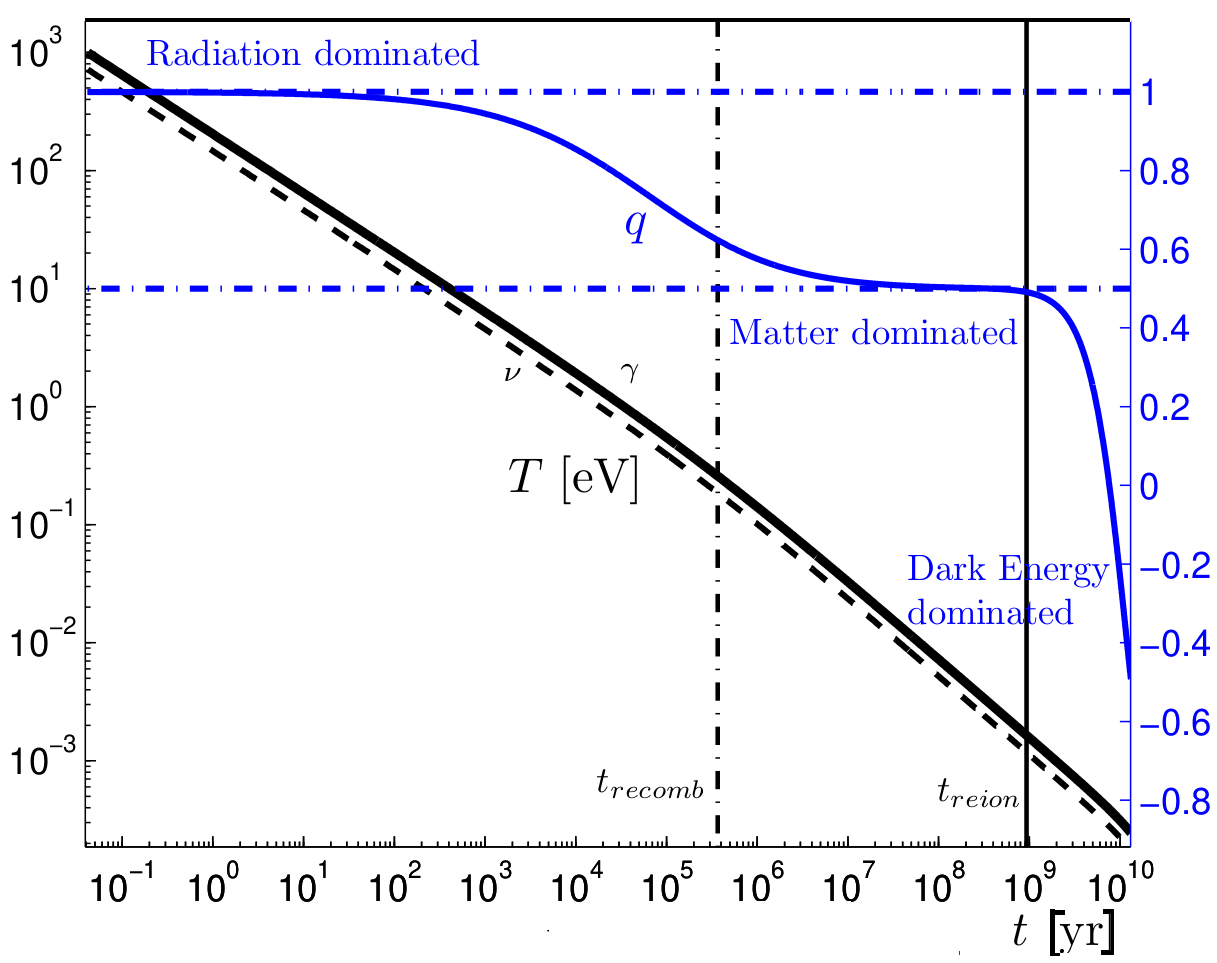
\includegraphics[width=0.88\linewidth]{01-introduction/Figures/Tqtoday.png}}
\caption{Deceleration parameter (blue lines, right hand scale) shows  transitions in the composition of the Universe as a function of time. The left hand scale indicates the corresponding $T$, dashed is the lower value for neutrinos. Vertical lines indicate recombination anr reionization conditions. Matter dominated Universe begins near recombination and ends right at the edge of reionization.  Adapted from~Ref.\,\cite{Rafelski:2013yka}
\label{fig:today} }
\end{figure}
%%%%%%%%%%%%%%%%%%%%%%%%%%%%%%%%%%%%%%%

On left axis in \rf{fig:today}  we see temperature $T$\,[eV] while on right axis (blue) we see the deceleration parameter $q$. The horizontal dot-dashed lines show the pure radiation-dominated value of $q=1$ and the matter-dominated value of $q=1/2$. The expansion in this era starts off as radiation-dominated. We see relatively long transitions to matter-dominated domain starting around $T=\mathcal{O}(300\eV)$ and  ending at $T=\mathcal{O}(10\eV)$. Thereafter begins the transition to a dark energy dominated era which is in full swing already at  $T=\mathcal{O}(1\eV)$. $q$ changes sign near to  $T=\mathcal{O}(200\meV)$. Today $q=-0.5$ indicates we are still in the midst of a rapid transition to dark energy dominated regime. 

The vertical dot-dashed lines in \rf{fig:today} show the time of recombination at $T\simeq0.25\eV$, when the Universe became transparent to photons, and reionization at $T\simeq {\cal O}(1\meV)$, when hydrogen in the Universe was again ionized due to light from the first galaxies~\cite{Zaroubi:2012in} is also shown.  The usefulness of $q$ to predict present day value of Hubble parameter is even better appreciated noting that we can easily  integrate \req{eq:Hdot} 
\beqn\label{eq:HdotInt}
H(t)=\frac{H_i}{1+H_i\int_{t_i}^{t}(1+q)dt}=
\frac{H_i}{1+1.5\,H_i\int_{t_i}^{t}(1+P/\rho)dt}\,.
\eeqn
We see, given an initial (measured) value $H_i$ in an epoch after free electrons disappeared (recombination epoch), that the time dependence of $q$ or equivalently, $P/\rho$, seen \rf{fig:today} impacts decisively the current epoch $H(t_0)=H_0$. To achieve an increase $H$ in current epoch beyond what is expected all it takes is to make $q$ a bit more negative, said differently diminish the (radiation) pressure, for example by reconsidering properties of the neutrino fluid in the Universe. We conclude that it is important to understand the particle content of the Universe which we used to construct these results in order to understand the riddle of the Hubble value tension.

\rf{fig:today1} shows the Hubble parameter $H$\,[s$^{-1}$] (left, black) and redshift $z+1\equiv a_0/a(t)$ (right, blue).  There is a visible deviation from a power law behavior due to the transitions from radiation to matter dominated and from matter to dark energy dominated expansion we saw in \rf{fig:today}.   

%%%%%%%%%%%%%%%%%%%%%%%%%%%%%%%%%%%%%%%
\begin{figure}
\centerline{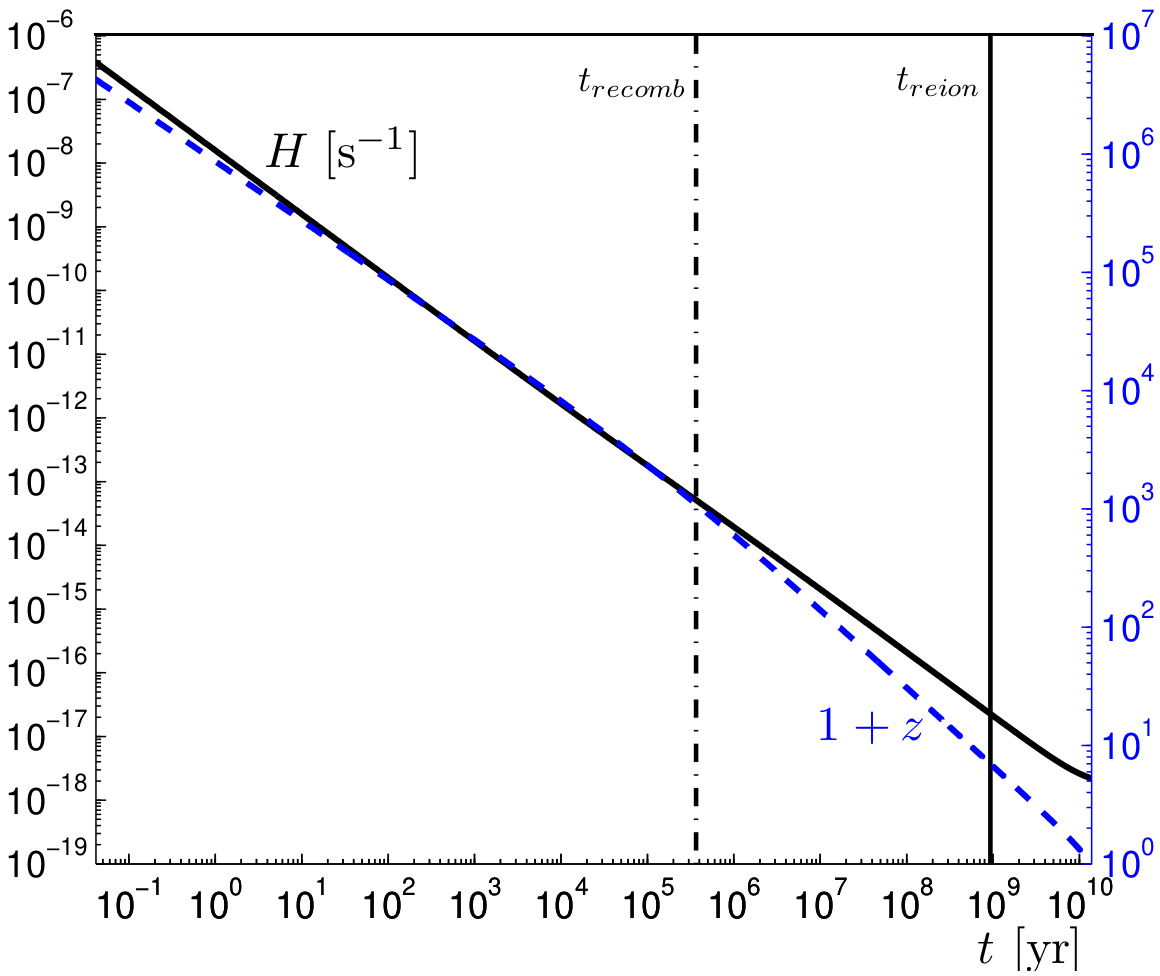
\includegraphics[width=0.88\linewidth]{01-introduction/Figures/Hztoday.png}}
\caption{Temporal evolution of the Hubble parameter $H$ (in units 1/s] (left hand scale) and of redshift $1+z$ (right hand scale, blue). Adapted from~Ref.\,\cite{Rafelski:2013yka} 
\label{fig:today1} }
\end{figure}
%%%%%%%%%%%%%%%%%%%%%%%%%%%%%%%%%%%%%%%


%%%%%%%%%%%%%%%%%%%%%%%%%%%%%
\paragraph{Relation between time and temperature}
Considering the comoving entropy conservation, we have
\begin{align}
S=\sigma V\propto g^s_\ast T^3a^3=\mathrm{constant},
\end{align}
where $g^s_\ast$ is the entropy degree of freedom and $a$ is the scale factor. Differentiating the entropy with respect to time $t$ we obtain
\begin{align}
\left[\frac{\dot{T}}{g^s_\ast}\frac{dg^s_\ast}{dT}+3\frac{\dot{T}}{T}+3\frac{\dot{a}}{a}\right]g^s_\ast T^3a^3=0,\qquad \dot{T}=\frac{dT}{dt}.
\end{align}
Solving $dT/dt$ and taking the integral, the relation between time and temperature in early universe can be written as
\begin{align}\label{time}
t(T)=t_0-\int^T_{T_0}dT\frac{1}{HT}\left[1+\frac{T}{3g^s_\ast}\frac{dg^s_\ast}{dT}\right],\qquad H^2=\frac{8\pi G_N}{3}\rho_{tot}
\end{align}
where $T_0$ and $t_0$ represent the initial temperature and time respectively, $H$ is the Hubble parameter and $\rho_{tot}$ is the total energy density in early Universe. From Eq. (\ref{time}) we see that the cosmic time depends on the entropy degrees of freedom $g^\ast_s$, which are characterized by the relativistic components in the early Universe. In the temperature range we consider  $T>0.02\,\mathrm{MeV}$ the Universe is radiation-dominated and non of elements of $\Lambda$CDM model is needed in this epoch.   
 

%%%%%%%%%%%%%%%%%%%%%%%%%%%%%%%%%%%%%%
%\subsection{Particle and plasma composition of the Universe} \label{ssec:ParticleU} 

Using the particle inventory in the Universe described above we can obtain explicit form of time-temperature relation. In \rf{Fig:Overview} the evolving particle inventory is discussed  showing both time and temperature: The black line presents relation between time $t$\,[sec] and temperature $T$\,[MeV] during the first hour of the evolution of the Univere, reaching to the temperature $T=10$\,keV. Vertical and horizontal lines indicate some characteristic events related to Universe particle inventory as marked. All of these will be discussed in this work. 
%%%%%%%%%%%%%%%%%%%%%%%%%%%%%%%%%%%%%%%
\begin{figure}
\centerline{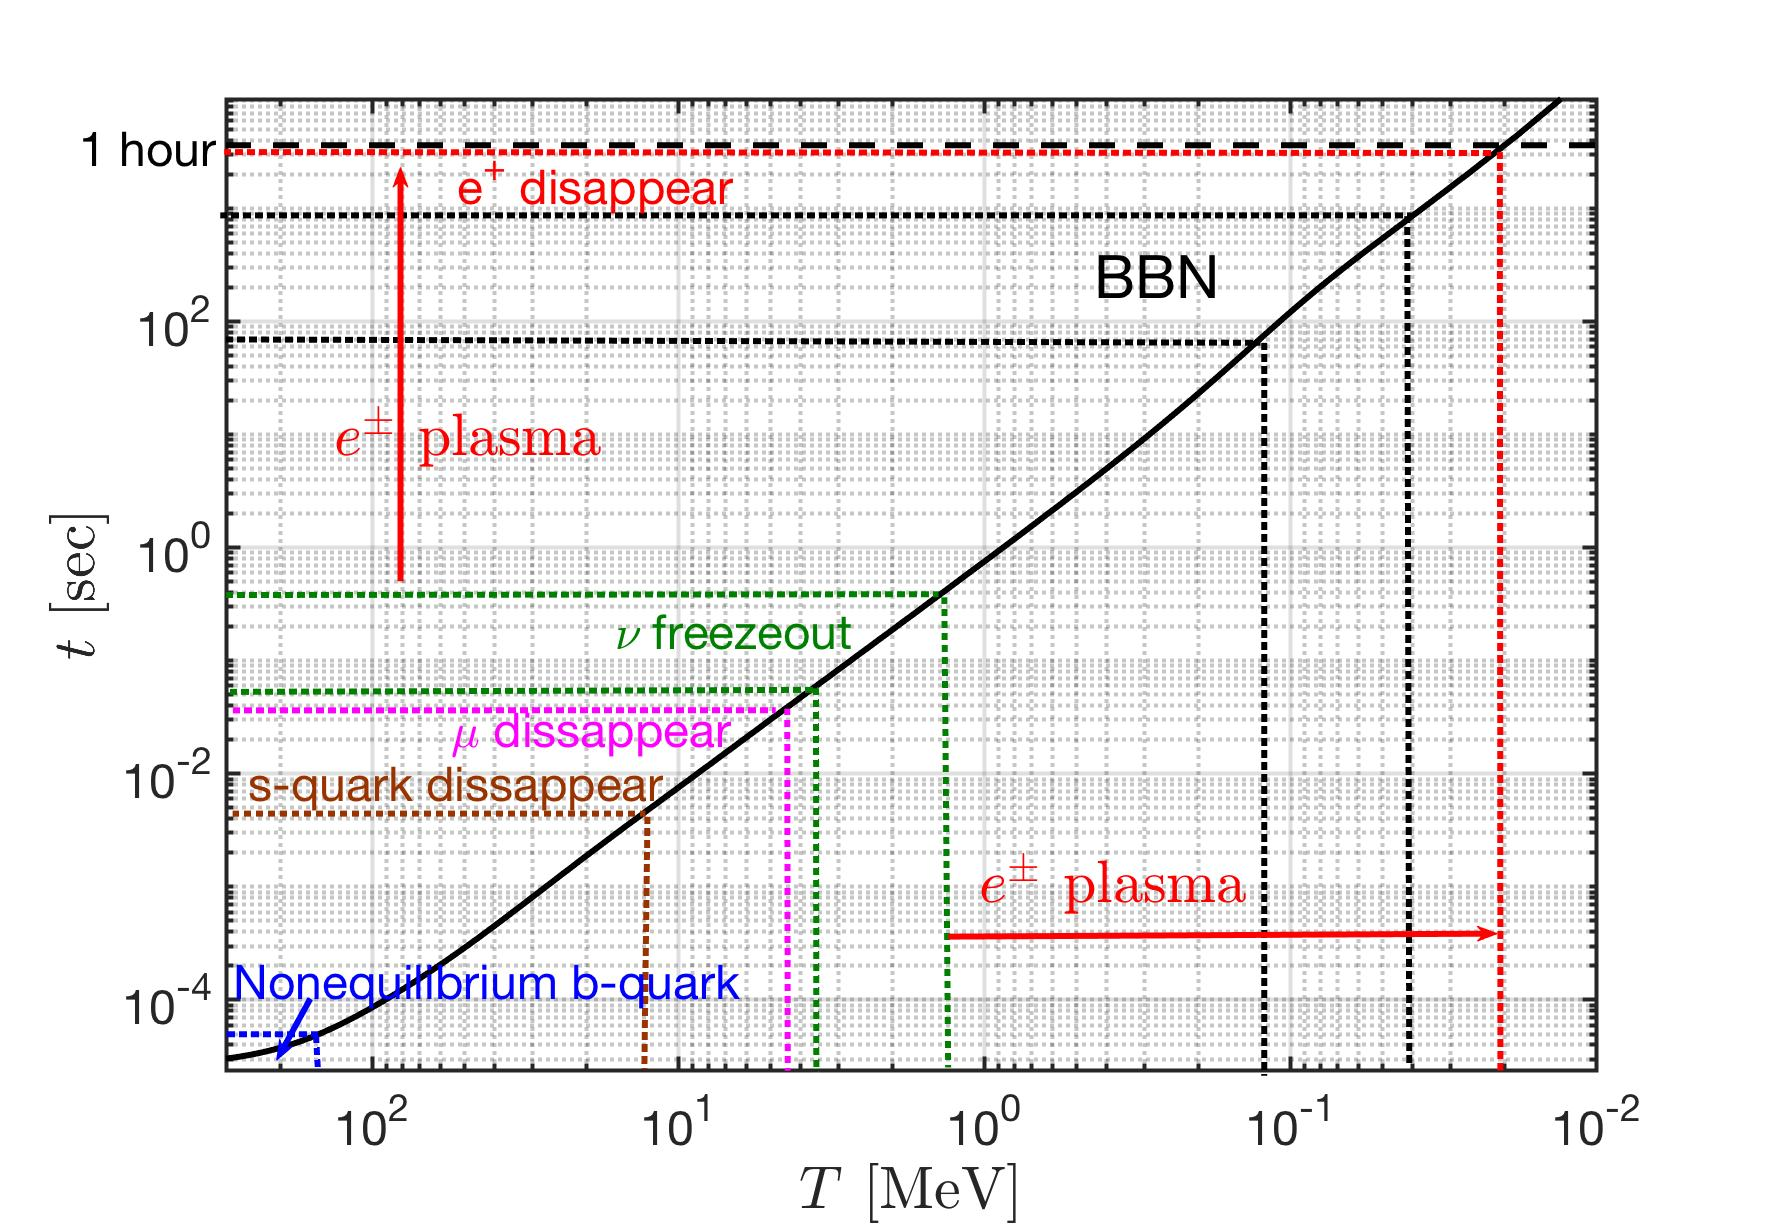
\includegraphics[width=\textwidth,width=\linewidth]{01-introduction/Figures/CosmicTimeTemperature.jpg}}
 \caption{The relation between time and temperature in the first hour of the Universe beginning shortly before QGP hadronization $300\,\mathrm{MeV}>T>0.02\,\mathrm{MeV} $ and ending with antimatter disappearance. Temperature/time range for several key events is indicated. Adapted from the thesis of C.T. Yang \cite{Yang:2024ret}}
 \label{Fig:Overview}
\end{figure}
%%%%%%%%%%%%%%%%%%%%%%%%%%%%%%%%%%%%%%%

%%%%%%%%%%%%%%%%%%%%%%%%%%%%%
\paragraph{The baryon-per-entropy density ratio}
An important assumption allowing us to explore the early Universe evolution is that following on the era of matter genesis both baryon and entropy content is conserved in the comoving volume. Both baryon and entropy density scale with the third power of the expansion parameter $a(t)$. Therefore the ratio of baryon number density to visible matter entropy density remains constant throughout the evolution of universe. We have \index{baryon per entropy ratio}
\begin{align}
\frac{n_B-n_{\overline{B}}}{\sigma}= \left.\frac{n_B-n_{\overline{B}}}{ \sigma}\right|_{t_0}=\mathrm{Const.}\;
\end{align}
The subscript $t_0$ denotes the present day condition, and $\sigma$ is the total entropy density.
The observation gives the present baryon-to-photon ratio ~\cite{ParticleDataGroup:2022pth} $5.8 \times 10^{-10} \leqslant(n_B-n_{\overline{B}})/n_\gamma\leqslant6.5\times10^{-10}$. This small value quantifies the matter-antimatter asymmetry in the present day Universe, and allows the determination of the present value of baryon per entropy ratio~\cite{Rafelski:2019twp,Fromerth:2002wb,Fromerth:2012fe}:
\begin{align}\label{BaryonEntropyRatio}
\left.\frac{n_B-n_{\overline{B}}}{ \sigma}\right|_{t_0}=\eta\left(\frac{n_\gamma}{\sigma_\gamma+\sigma_\nu}\right)_{\!t_0}\!\!\!\!=(8.69\pm0.05)\!\!\times\!\!10^{-11},\qquad \eta=\frac{(n_B-n_{\overline{B}})}{n_\gamma},
\end{align}
where the $\eta=(6.12\pm0.04)\times10^{-10}$~\cite{ParticleDataGroup:2022pth} is used in calculation. To obtain the ratio, we consider that the Universe today is dominated by photons and free-streaming massless neutrinos~\cite{Birrell:2012gg}, and $\sigma_\gamma$ and $\sigma_\nu$ are the entropy densities for photon and neutrino respectively. We have
\begin{align}
    \frac{\sigma_\nu}{\sigma_\gamma}=\frac{7}{8}\,\frac{g_\nu}{g_\gamma}\left(\frac{T_\nu}{T_\gamma}\right)^3\,,\qquad\frac{T_\nu}{T_\gamma}=\left(\frac{4}{11}\right)^{1/3}
\end{align}
and the entropy-per-particle for massless bosons and fermions are given by~\cite{Fromerth:2012fe}
\begin{align}
s/n|_\mathrm{boson}\approx 3.60\,,\qquad
s/n|_\mathrm{fermion}\approx 4.20\,.
\end{align}
However, from the neutrino oscillation experiment, we know that the the neutrinos are not massless particles. 
The mass differences between neutrino mass eigenstates are~\cite{ParticleDataGroup:2022pth}:
\begin{align}
&\Delta{m}_{21}^2=7.39^{+0.21}_{-0.20}\times10^{-5}\,\mathrm{eV}^2,\\
&\Delta{m}_{32}^2=2.45^{+0.03}_{-0.03}\times10^{-3}\,\mathrm{eV}^2.
\end{align}
Neutrino mass eigenvalues can be ordered in the normal mass hierarchy ($m_1\ll m_2<m_3$) or inverted mass hierarchy ($m_3\ll m_1<m_2$). All three mass states remained relativistic until the temperature dropped below their rest mass. These results allow for the possibility that one mass eigenstate or two mass eigenstates of neutrinos may become non-relativistic today, which can affect the baryon-per-entropy ratio.


%%%%%%%%%%%%%%%%%%%%%%%%%%%%%%%%%%%%%%%%%%%%
\paragraph{Reheating History of the Universe}
%\label{Eralink}

At times where dimensional scales are irrelevant, entropy conservation means that temperature scales inversely with the scale factor $a(t)$. This follows from the only contributing scale being $T$ and therefore by dimensional counting $ \rho\simeq 3P \propto T^4$. However, as the temperature drops and at their respective $m\simeq T$ scales, successively less massive particles annihilate and disappear from the thermal Universe. Their entropy reheats the other degrees of freedom and thus in the process, the entropy originating in a massive degree of freedom is shifted into the effectively massless degrees of freedom that still remain. This causes the $T\propto 1/a(t)$ scaling to break down; during each of these `reorganization' periods the drop in temperature is slowed by the concentration of entropy in fewer degrees of freedom, leading to a change in the reheating ratio, $R$, defined as
\begin{equation}\label{redshiftratio}
R\equiv \frac{1+z}{ T_\gamma/T_{\gamma,0}}, \qquad 1+z\equiv \frac{a_{0}}{a(t)}.
\end{equation}
The reheating ratio connects the photon temperature redshift to the geometric redshift, where $a_0$ is the scale factor today (often normalized to $1$) and quantifies the deviation from the scaling relation between $a(t)$ and $T$.

As we will see, the change in $R$ can be computed by the drop in the number of degrees of freedom. At a temperature on the order of the top quark mass, when all standard model particles were in thermal equilibrium, the Universe was pushed apart by 28 bosonic and 90 fermionic degrees of freedom. The total number of degrees of freedom can be computed as follows. 

For bosons we have the following: the doublet of charged Higgs particles has $4=2\times2=1+3$ degrees of freedom -- three will migrate to the longitudinal components of $W^\pm, Z$ when the electro-weak vacuum freezes and the EW symmetry breaking arises, while one is retained in the one single dynamical charge neutral Higgs component. In the massless stage, the SU(2)$\times$U(1) theory has 4$\times$2=8 gauge degrees of freedom where the first coefficient is the number of particles $(\gamma, Z, W^\pm)$ and each massless gauge boson has two transverse polarizations. Adding in $8_c\times2_s=16$ gluonic degrees of freedom we obtain 4+8+16=28 bosonic degrees of freedom. 

The count of fermionic degrees of freedom includes three $f$ families, two spins $s$, another factor two for particle-antiparticle duality. We have in each family of flavors a doublet of $2\times 3_c$ quarks, 1-lepton and 1/2 neutrinos (due left-handedness which was not implemented counting spin). Thus we find that a total $3_f\times 2_p\times 2_s\times(2\times 3_c+1_l+1/2_\nu)=90$ fermionic degrees of freedom. We further recall that massless fermions contribute 7/8 of that of bosons in both pressure and energy density. Thus the total number of massless Standard Model particles at a temperature above the top quark mass scale, referring by convention to bosonic degrees of freedom, is $g_{\rm SM}=28+90\times 7/8=106.75$ 



In \rf{fig:dof} we show the cube of the reheating ratio \req{redshiftratio} as a function of photon temperature $T_\gamma$ from the primordial high temperature early Universe on the right to the present on the left, where $R$ must be by definition unity. The periods of change seen in Figure \ref{fig:dof} come when the temperature crosses the mass of a particle species that is in equilibrium. One can see drops corresponding to the disappearance of particles as indicated. After $e^+e^-$ annihilation on the left, there are no significant degrees of freedom remaining to annihilate and feed entropy into photons, and so $R$ remains constant until today. We show the result using a Fermi gas model with a very rough model for the QGP phase transition and hadronization period near $O(100\MeV)$. The fermi gas model is a poor approximation above the QGP phase transition; a more precise model using lattice QCD, see e.g.~\cite{Borsanyi:2013bia}, together with a high temperature perturbative QCD expansion, see e.g.~\cite{Letessier:2002ony}, would be needed to improve on this situation but the details do not impact the neutrino freeze-out period near $1\MeV$ which is our primary concern, and so we do not consider these issues further here.

%%%%%%%%%%%%%%%%%%%%%%%%%%%%%%%%%%%%%%%
\begin{figure} 
\centerline{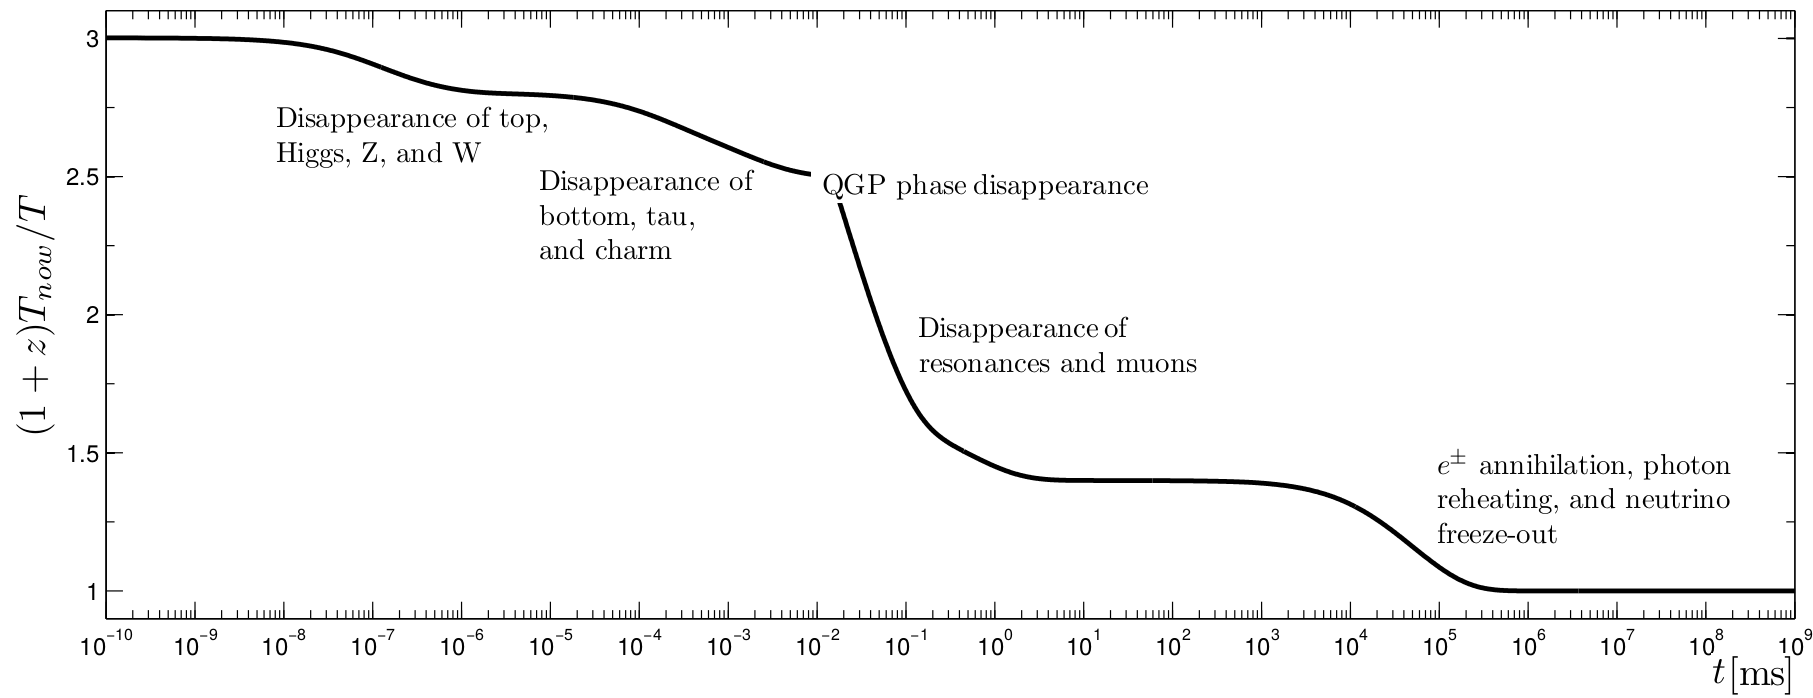
\includegraphics[height=5.2cm]{01-introduction/Figures/DOFtime.png}}
\caption{Disappearance of degrees of freedom throughout the history of the Universe as a function of time since Big-Bang in milliseconds. The Universe volume inflated approximately by a factor of 27 above the naive thermal red shift scale as massive particles disappeared successively from the inventory. Adopted from the thesis of J.\,Birrell~\cite{Birrell:2014ona} \label{fig:dof}}
 \end{figure}
%%%%%%%%%%%%%%%%%%%%%%%%%%%%%%%%%%%%%%%



As long as the dynamics are at least approximately entropy conserving, the total drop in $R$ is entirely determined by entropy conservation. Namely, the magnitude of the drop in $R$ \rf{fig:dof} is a measure of the number of degrees of freedom that have disappeared from the Universe. Consider two times $t_1$ and $t_2$ at which all particle species that have not yet annihilated are effectively massless. By conservation of comoving entropy and scaling $T\propto 1/a$ we have
\begin{equation}\label{r_ratio}
1=\frac{a_1^3S_{1}}{a_2^3 S_2}=\frac{a_1^3\sum_ig_i T_{i,1}^3}{a_2^3\sum_j g_j T_{j,2}^3},\qquad \left(\frac{R_1}{R_2}\right)^3=\frac{\sum_ig_i (T_{i,1}/T_{\gamma,1})^3}{\sum_j g_j (T_{j,2}/T_{\gamma,2})^3}
\end{equation}
where the sums are over the total number of degrees of freedom present at the indicated time and the degeneracy factors $g_i$ contain the $7/8$ factor for fermions. In the second form we divided the numerator and denominator by $a_{0}T_{\gamma,0}$. We distinguish between the temperature of each particle species and our reference temperature, the photon temperature. This is important since today neutrinos are colder than photons, due to photon reheating from $e^\pm$ annihilation occurring after neutrinos decoupled (this is only an approximation, a point we will study in detail in subsequent chapters). By conservation of entropy one obtains the neutrino to photon temperature ratio of
\begin{equation}\label{T_nu_T_gamma}
T_\nu/T_\gamma=({4}/{11})^{1/3}.
\end{equation}
We will call this the reheating ratio in the decoupled limit. 

Using \req{r_ratio} we compute the total drop in $R^3$ shown in Figure \ref{fig:dof}. At $T=T_\gamma=\mathcal{O}(100\GeV)$ the number of active degrees of freedom is slightly below $g_{\rm SM}=106.75$ due to the partial disappearance of top quarks, but this approximation will be good enough for our purposes. At this time, all the species are in thermal equilibrium with photons and so $T_{i,1}/T_{\gamma,1}=1$ for all $i$. Today we have $2$ photon and $7/8\times 6$ neutrino degrees of freedom and a neutrino to photon temperature ratio \req{T_nu_T_gamma}. Therefore we have
\begin{equation}
\left(\frac{R_{100GeV}}{R_{now}}\right)^3= \frac{g_{SM}}{g_{\rm now}}=\frac{106.75}{2+\frac{7}{8}\times 6\times \frac{4}{11}}\approx 27.3
\end{equation}
which is the fractional change we see in the fermi gas model curve in Figure \ref{fig:dof} (as mentioned above, the QCD model is reduced due to interactions). The meaning of this factor is that the Universe approximately inflated by a factor 27 above the thermal red shift scale as massive particles disappeared successively from the inventory. 

From the perspective of reheating, the history of the Universe from the end of $e^\pm$ annihilation until today has been uneventful. 

We can shed additional light on this period and others by looking at the composition of the Universe as a function of temperature


In Figure \ref{fig:energy_frac} we begin on the right at the end of the hadron era with the disappearance of muons and pions. This constitutes a reheating period, with energy and entropy from these particles being transferred to the remaining $e^\pm$, photon, neutrino plasma. Continuing to $T=O(1)$ MeV, we come to the annihilation of $e^\pm$ and the photon reheating period. Notice that only the photon energy density fraction increases here. As discussed above, a common simplifying assumption is that neutrinos are already decoupled at this time and hence do not share in the reheating process, leading to a difference in photon and neutrino temperatures \req{T_nu_T_gamma}.

After passing through a long period, from $T=O(1)$ MeV until $T=O(1)$ eV, where the energy density is dominated by photons and free-streaming neutrinos, we then come to the beginning of the matter dominated regime, where the energy density is dominated by dark matter and baryonic matter. This transition is the result of the redshifting of the photon and neutrino energy, $\rho\propto T^4$, whereas for non-relativistic matter $\rho\propto a^{-3}\propto T^3$. Note that our inclusion of neutrino mass causes the leveling out of the neutrino energy density fraction during this period, as compared to the continued redshifting of the photon energy.

Finally, as we move towards the present day CMB temperature of $T_{\gamma,0}=0.235$ meV on the left hand side, we have entered the dark energy dominated regime. For the present day values, we have used the fits from the Planck data~\cite{Planck:2018vyg,Planck:2015fie,Planck:2013pxb} of $69\%$ dark energy, $26\%$ dark matter and $5\%$ baryons (and zero spatial curvature). The photon energy density is fixed by the CMB temperature $T_{\gamma,0}$ and the neutrino energy density is fixed by $T_{\gamma,0}$ along with the photon to neutrino temperature ratio. Both constitute $<1\%$ of the current energy budget.

%%%%%%%%%%%%%%%%%%%%%%%%%%%%%%%%%%%%%%%%%%%%%%
%\subsubsection\label{recomb}
\paragraph{Looking back in time:}
In the following we use the mix of matter (31\%) and dark energy (69\%) with photon and neutrino backgrounds favored by the latest Planck results~\cite{Planck:2018vyg,Planck:2015fie,Planck:2013pxb}, where we gave two neutrino species mass of $m_\nu=30\meV$ and a third neutrino remains massless. This is a different mass value than used above and again, it is only for illustration-- other mass choices are possible within present day constraints and will impact to some degree where exactly matter dominance emerges from the radiative Universe. We presume that neutrino kinetic freeze-out completed before the onset of $e^\pm$-annihilation into photons, leading to the neutrino to photon temperature ratio \req{T_nu_T_gamma}. Again, this is a common simplifying assumption. Much of the remainder of this work will involve improving on this approximation, but for the purposes of this overview it is sufficient.

%%%%%%%%%%%%%%%%%%%%%%%%%%%%%%%%%%%%%%%%%
\paragraph{First look at neutrino freeze-out era} 
%\label{nudecoup}
%\paragraph{Neutrino freeze-out era:} 
The era separating the photon-neutrino-matter-dark energy Universe we just described from the end of the hadron Universe is quite complex in its evolution. We begin when the number of $e^\pm$-pairs has decayed to the same abundance as the number of baryons in the Universe at the temperature $T=\mathcal{O}(10\keV)$ and reach back to $T={\cal O}(30\MeV)$ where muons and pions are disappearing from the Universe.

%%%%%%%%%%%%%%%%%%%%%%%%%%%%%%%%%%%%%%%
\begin{figure}
\centerline{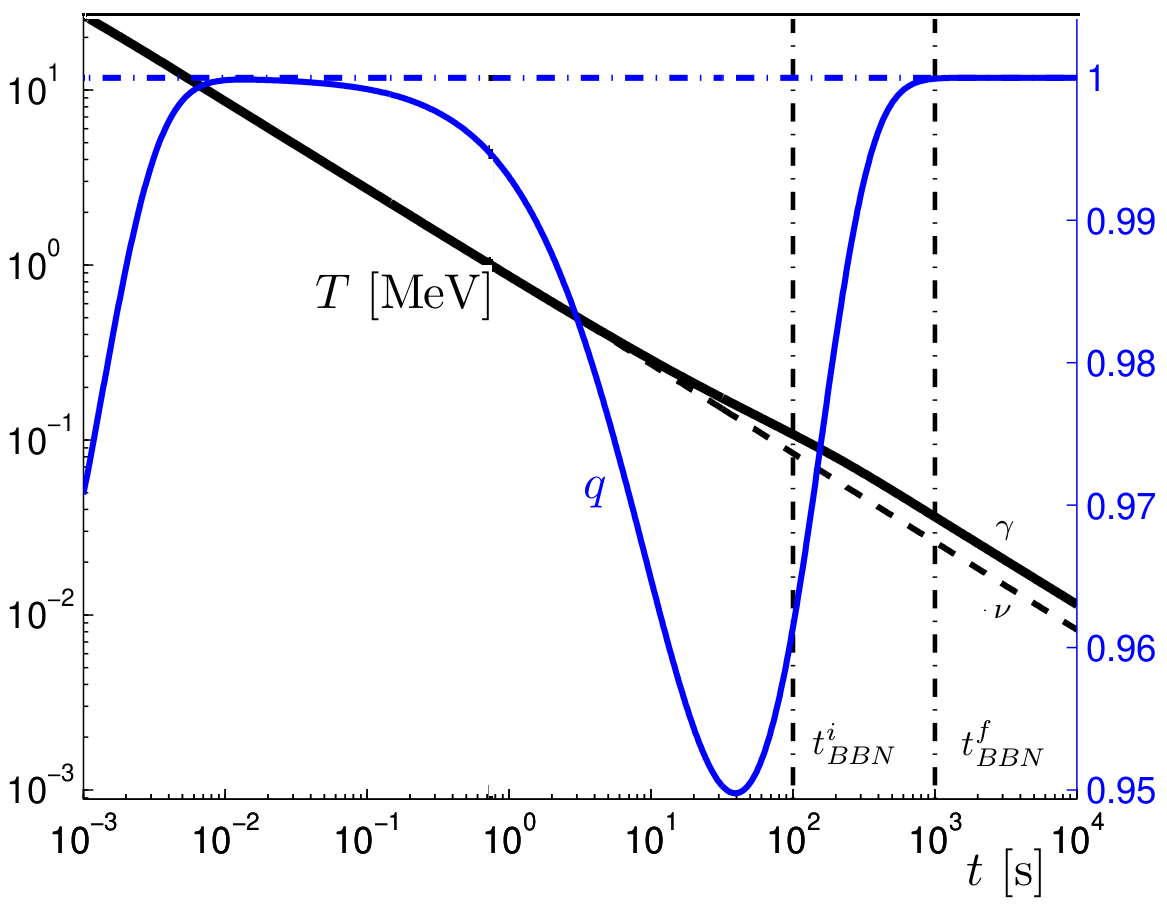
\includegraphics[width=0.90\textwidth]{01-introduction/Figures/TqBBN.png}}
\caption{The first hours in the lifespan of the Universe  from the end of baryon antimatter annihilation through BBN: Deceleration parameter $q$ (blue line, right hand scale) shows impact of emerging antimatter components; at millisecond scale antibrayonic matter and at 35 second scale positronic nonrelativistic matter appears. The left hand scale shows photon $\gamma$ temperature $T$ in eV, dashed is the emerging lower value for neutrino $\nu$ which are not reheated by $e^+e^-$ annihilation. Vertical lines bracket the BBN domain. Adopted from~Ref.\,\cite{Rafelski:2013yka}  
\label{fig:BBN}}
\end{figure}
%%%%%%%%%%%%%%%%%%%%%%%%%%%%%%%%%%%%%%%

%%%%%%%%%%%%%%%%%%%%%%%%%%%%%%%%%%%%%%%
\begin{figure}
\centerline{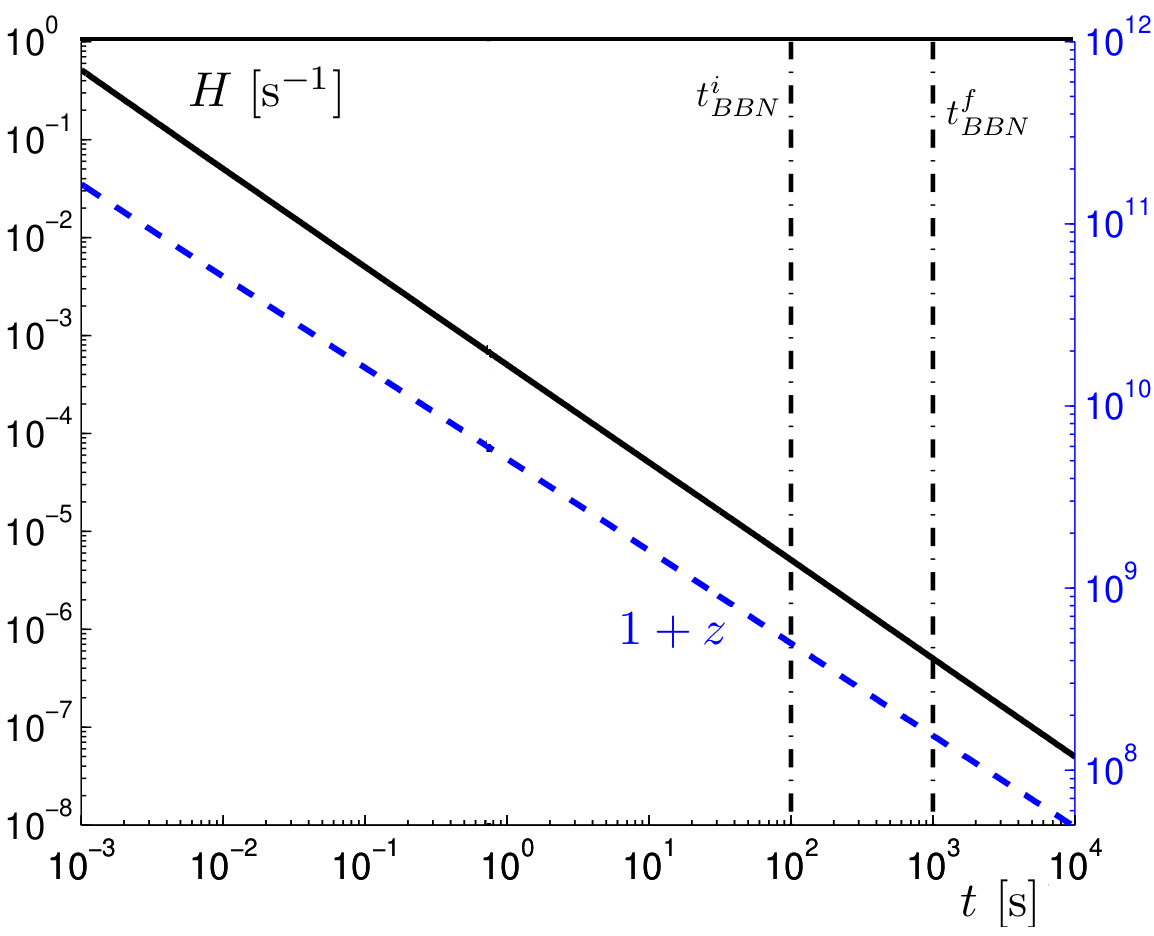
\includegraphics[width=0.90\linewidth]{01-introduction/Figures/HzBBN.png}} 
\caption{First hours in the evolution of the Universe: Hubble parameter $H$ in units [1/s] (left hand scale) and the redshift $1+z$ (right hand scale, blue) spanning the epoch from  the end of baryon antimatter annihilation through BBN, compare \rf{fig:BBN}. Adopted from~Ref.\,\cite{Rafelski:2013yka} 
\label{fig:BBN1}}
\end{figure}
%%%%%%%%%%%%%%%%%%%%%%%%%%%%%%%%%%%%%%%

 In \rf{fig:BBN} the horizontal dot-dashed line for $q=1$ shows the pure radiation dominated value with two exceptions. First, the presence of massive pions and muons reduce the value of $q$ near to the maximal temperature shown. Second, when the temperature is near the value of the electron mass, the $e^\pm$-pairs are not yet fully depleted but already sufficiently non-relativistic to cause another dip in $q$. These are not large drops; the expansion is still predominately radiation dominated. But $q$ provides a sensitive measure of when various mass scales become relevant and is a good indicator of the presence of a reheating period.

 The dashed line shows the neutrino temperature, which decouples from the $e^\pm$ and photon temperature at $T={\cal O}(1\MeV)$ when neutrinos freeze-out and begin free streaming. In \rf{fig:BBN} the unit of time is seconds and the range spans the domain from fractions of a millisecond to a few hours. After neutrino freeze-out we come to Big Bang Nucleosynthesis, the period when the lighter elements were synthesized in a hot but relatively dilute plasma~\cite{Iocco:2008va}. We left some time gap between this and the domain shown in Figure \ref{fig:today} describing the current era -- there is an uneventful evolution between the two domains. 
 